\documentclass[a4paper]{book}
\usepackage{a4wide}
\usepackage{makeidx}
\usepackage{graphicx}
\usepackage{multicol}
\usepackage{float}
\usepackage{listings}
\usepackage{color}
\usepackage{textcomp}
\usepackage{alltt}
\usepackage{times}
\usepackage{ifpdf}
\ifpdf
\usepackage[pdftex,
            pagebackref=true,
            colorlinks=true,
            linkcolor=blue,
            unicode
           ]{hyperref}
\else
\usepackage[ps2pdf,
            pagebackref=true,
            colorlinks=true,
            linkcolor=blue,
            unicode
           ]{hyperref}
\usepackage{pspicture}
\fi
\usepackage[utf8]{inputenc}
\usepackage{doxygen}
\lstset{language=C++,inputencoding=utf8,basicstyle=\footnotesize,breaklines=true,breakatwhitespace=true,tabsize=8,numbers=left }
\makeindex
\setcounter{tocdepth}{3}
\renewcommand{\footrulewidth}{0.4pt}
\begin{document}
\hypersetup{pageanchor=false}
\begin{titlepage}
\vspace*{7cm}
\begin{center}
{\Large JREngage }\\
\vspace*{1cm}
{\large Generated by Doxygen 1.7.1}\\
\vspace*{0.5cm}
{\small Mon May 9 2011 10:54:23}\\
\end{center}
\end{titlepage}
\clearemptydoublepage
\pagenumbering{roman}
\tableofcontents
\clearemptydoublepage
\pagenumbering{arabic}
\hypersetup{pageanchor=true}
\chapter{Janrain Engage for the iPhone, version 2}
\label{index}\hypertarget{index}{}\href{http://rpxnow.com/docs/iphone}{\tt Janrain Engage for iPhone SDK} makes it easy to include third party authentication and social publishing in your iPhone app. This Objective-\/C library includes the same key features as our web version, as well as additional features created specifically for the mobile platform. With as few as three lines of code, you can authenticate your users with their accounts on Google, Yahoo!, Facebook, etc., and they can immediately publish their activities to multiple social networks, including Facebook, Twitter, LinkedIn, MySpace, and Yahoo, through one simple interface.

Beyond authentication and social sharing, the latest release of the Engage for iPhone SDK now allows mobile apps to:
\begin{DoxyItemize}
\item Share content, activities, game scores or invitations via Email or SMS
\item Customize the login experience by displaying native and social login options on the same screen
\item Track popularity and click through rates on various links included in the shared email message with automatic URL shortening for up to 5 URLs
\item Provide an additional level of security with forced re-\/authentication when users are about to make a purchase or conduct a sensitive transaction
\item Configure and maintain separate lists of providers for mobile and web apps
\item Match the look and feel of the iPhone app with customizable background colors, images, and navigation bar tints
\end{DoxyItemize}

Before you begin, you need to have created a \href{https://rpxnow.com/signup_createapp_plus}{\tt Janrain Engage application}, which you can do on \href{http://rpxnow.com}{\tt http://rpxnow.com}

For an overview of how the library works and how you can take advantage of the library's features, please see the \href{http://rpxnow.com/docs/iphone#user_experience}{\tt \char`\"{}Overview\char`\"{}} section of our documentation.

To begin using the SDK, please see the \href{http://rpxnow.com/docs/iphone#quick}{\tt \char`\"{}Quick Start Guide\char`\"{}}.

For more detailed documentation of the library's API, you can use the \href{http://rpxnow.com/docs/iphone_api/annotated.html}{\tt \char`\"{}JREngage API\char`\"{}} documentation. 
\chapter{Providers}
\label{Providers}
\hypertarget{Providers}{}
\hypertarget{_providers_basicProviders}{}\section{List of Providers}\label{_providers_basicProviders}
Here is a list of possible strings that the argument (NSString$\ast$)provider can be when used in the authentication methods:
\begin{DoxyItemize}
\item \char`\"{}aol\char`\"{}
\item \char`\"{}blogger\char`\"{}
\item \char`\"{}facebook\char`\"{}
\item \char`\"{}flickr\char`\"{}
\item \char`\"{}google\char`\"{}
\item \char`\"{}hyves\char`\"{}
\item \char`\"{}linkedin\char`\"{}
\item \char`\"{}live\_\-id\char`\"{}
\item \char`\"{}livejournal\char`\"{}
\item \char`\"{}myopenid\char`\"{}
\item \char`\"{}myspace\char`\"{}
\item \char`\"{}netlog\char`\"{}
\item \char`\"{}openid\char`\"{}
\item \char`\"{}paypal\char`\"{}
\item \char`\"{}twitter\char`\"{}
\item \char`\"{}verisign\char`\"{}
\item \char`\"{}yahoo\char`\"{}
\end{DoxyItemize}

\begin{DoxyNote}{Note}
As your Engage application is limited by the number of providers it may use, you may only see a subset of this list.
\end{DoxyNote}
\hypertarget{_providers_socialProviders}{}\section{List of Social Providers}\label{_providers_socialProviders}
Here is a list of possible strings that the argument (NSString$\ast$)provider can be when used in the social publishing methods:
\begin{DoxyItemize}
\item \char`\"{}facebook\char`\"{}
\item \char`\"{}linkedin\char`\"{}
\item \char`\"{}myspace\char`\"{}
\item \char`\"{}twitter\char`\"{}
\item \char`\"{}yahoo\char`\"{}
\end{DoxyItemize}

\begin{DoxyNote}{Note}
As your Engage application is limited by the number of providers it may use, you may only see a subset of this list. 
\end{DoxyNote}

\chapter{Class Index}
\section{Class Hierarchy}
This inheritance list is sorted roughly, but not completely, alphabetically:\begin{DoxyCompactList}
\item \contentsline{section}{com.janrain.android.engage.utils.Archiver}{\pageref{classcom_1_1janrain_1_1android_1_1engage_1_1utils_1_1_archiver}}{}
\item \contentsline{section}{com.janrain.android.engage.types.JRActionLink}{\pageref{classcom_1_1janrain_1_1android_1_1engage_1_1types_1_1_j_r_action_link}}{}
\item \contentsline{section}{com.janrain.android.engage.types.JRActivityObject}{\pageref{classcom_1_1janrain_1_1android_1_1engage_1_1types_1_1_j_r_activity_object}}{}
\item \contentsline{section}{com.janrain.android.engage.types.JRDictionary}{\pageref{classcom_1_1janrain_1_1android_1_1engage_1_1types_1_1_j_r_dictionary}}{}
\item \contentsline{section}{com.janrain.android.engage.JREngage}{\pageref{classcom_1_1janrain_1_1android_1_1engage_1_1_j_r_engage}}{}
\item \contentsline{section}{com.janrain.android.engage.JREngageDelegate}{\pageref{interfacecom_1_1janrain_1_1android_1_1engage_1_1_j_r_engage_delegate}}{}
\item \contentsline{section}{com.janrain.android.engage.JREngageError}{\pageref{classcom_1_1janrain_1_1android_1_1engage_1_1_j_r_engage_error}}{}
\item \contentsline{section}{com.janrain.android.engage.ui.JRLandingActivity}{\pageref{classcom_1_1janrain_1_1android_1_1engage_1_1ui_1_1_j_r_landing_activity}}{}
\item \contentsline{section}{com.janrain.android.engage.types.JRMediaObject}{\pageref{classcom_1_1janrain_1_1android_1_1engage_1_1types_1_1_j_r_media_object}}{}
\begin{DoxyCompactList}
\item \contentsline{section}{com.janrain.android.engage.types.JRFlashMediaObject}{\pageref{classcom_1_1janrain_1_1android_1_1engage_1_1types_1_1_j_r_flash_media_object}}{}
\item \contentsline{section}{com.janrain.android.engage.types.JRImageMediaObject}{\pageref{classcom_1_1janrain_1_1android_1_1engage_1_1types_1_1_j_r_image_media_object}}{}
\item \contentsline{section}{com.janrain.android.engage.types.JRMp3MediaObject}{\pageref{classcom_1_1janrain_1_1android_1_1engage_1_1types_1_1_j_r_mp3_media_object}}{}
\end{DoxyCompactList}
\item \contentsline{section}{com.janrain.android.engage.ui.JRProvidersActivity}{\pageref{classcom_1_1janrain_1_1android_1_1engage_1_1ui_1_1_j_r_providers_activity}}{}
\item \contentsline{section}{com.janrain.android.engage.ui.JRPublishActivity}{\pageref{classcom_1_1janrain_1_1android_1_1engage_1_1ui_1_1_j_r_publish_activity}}{}
\item \contentsline{section}{com.janrain.android.engage.ui.JRUserInterfaceMaestro}{\pageref{classcom_1_1janrain_1_1android_1_1engage_1_1ui_1_1_j_r_user_interface_maestro}}{}
\item \contentsline{section}{com.janrain.android.engage.ui.JRWebViewActivity}{\pageref{classcom_1_1janrain_1_1android_1_1engage_1_1ui_1_1_j_r_web_view_activity}}{}
\item \contentsline{section}{com.janrain.android.engage.utils.ListUtils}{\pageref{classcom_1_1janrain_1_1android_1_1engage_1_1utils_1_1_list_utils}}{}
\item \contentsline{section}{com.janrain.android.engage.ui.SharedLayoutHelper}{\pageref{classcom_1_1janrain_1_1android_1_1engage_1_1ui_1_1_shared_layout_helper}}{}
\item \contentsline{section}{com.janrain.android.engage.utils.StringUtils}{\pageref{classcom_1_1janrain_1_1android_1_1engage_1_1utils_1_1_string_utils}}{}
\end{DoxyCompactList}

\chapter{Class Index}
\section{Class List}
Here are the classes, structs, unions and interfaces with brief descriptions:\begin{DoxyCompactList}
\item\contentsline{section}{\hyperlink{classcom_1_1janrain_1_1android_1_1engage_1_1ui_1_1_j_r_landing_activity_1_1_finish_receiver}{JRLandingActivity.FinishReceiver} }{\pageref{classcom_1_1janrain_1_1android_1_1engage_1_1ui_1_1_j_r_landing_activity_1_1_finish_receiver}}{}
\item\contentsline{section}{\hyperlink{classcom_1_1janrain_1_1android_1_1engage_1_1ui_1_1_j_r_providers_activity_1_1_finish_receiver}{JRProvidersActivity.FinishReceiver} }{\pageref{classcom_1_1janrain_1_1android_1_1engage_1_1ui_1_1_j_r_providers_activity_1_1_finish_receiver}}{}
\item\contentsline{section}{\hyperlink{classcom_1_1janrain_1_1android_1_1engage_1_1ui_1_1_j_r_publish_activity_1_1_finish_receiver}{JRPublishActivity.FinishReceiver} }{\pageref{classcom_1_1janrain_1_1android_1_1engage_1_1ui_1_1_j_r_publish_activity_1_1_finish_receiver}}{}
\item\contentsline{section}{\hyperlink{classcom_1_1janrain_1_1android_1_1engage_1_1ui_1_1_j_r_web_view_activity_1_1_finish_receiver}{JRWebViewActivity.FinishReceiver} }{\pageref{classcom_1_1janrain_1_1android_1_1engage_1_1ui_1_1_j_r_web_view_activity_1_1_finish_receiver}}{}
\item\contentsline{section}{\hyperlink{classcom_1_1janrain_1_1android_1_1engage_1_1types_1_1_j_r_action_link}{JRActionLink} (A link a user can use to take action on an activity update on the provider )}{\pageref{classcom_1_1janrain_1_1android_1_1engage_1_1types_1_1_j_r_action_link}}{}
\item\contentsline{section}{\hyperlink{classcom_1_1janrain_1_1android_1_1engage_1_1types_1_1_j_r_activity_object}{JRActivityObject} (An activity object you create, populate, and post to the user's activity stream )}{\pageref{classcom_1_1janrain_1_1android_1_1engage_1_1types_1_1_j_r_activity_object}}{}
\item\contentsline{section}{\hyperlink{classcom_1_1janrain_1_1android_1_1engage_1_1types_1_1_j_r_dictionary}{JRDictionary} }{\pageref{classcom_1_1janrain_1_1android_1_1engage_1_1types_1_1_j_r_dictionary}}{}
\item\contentsline{section}{\hyperlink{classcom_1_1janrain_1_1android_1_1engage_1_1_j_r_engage}{JREngage} (Main API for interacting with the Janrain Engage for iPhone library )}{\pageref{classcom_1_1janrain_1_1android_1_1engage_1_1_j_r_engage}}{}
\item\contentsline{section}{\hyperlink{interfacecom_1_1janrain_1_1android_1_1engage_1_1_j_r_engage_delegate}{JREngageDelegate} (The \hyperlink{interfacecom_1_1janrain_1_1android_1_1engage_1_1_j_r_engage_delegate}{JREngageDelegate} protocol is adopted by an object that wishes to receive notifications when and information about a user that authenticates with your application and publishes activities to their social networks )}{\pageref{interfacecom_1_1janrain_1_1android_1_1engage_1_1_j_r_engage_delegate}}{}
\item\contentsline{section}{\hyperlink{classcom_1_1janrain_1_1android_1_1engage_1_1_j_r_engage_error}{JREngageError} }{\pageref{classcom_1_1janrain_1_1android_1_1engage_1_1_j_r_engage_error}}{}
\item\contentsline{section}{\hyperlink{classcom_1_1janrain_1_1android_1_1engage_1_1types_1_1_j_r_flash_media_object}{JRFlashMediaObject} (Flash object to be included in a post to a user's stream )}{\pageref{classcom_1_1janrain_1_1android_1_1engage_1_1types_1_1_j_r_flash_media_object}}{}
\item\contentsline{section}{\hyperlink{classcom_1_1janrain_1_1android_1_1engage_1_1types_1_1_j_r_image_media_object}{JRImageMediaObject} (Image object to be included in a post to a user's stream )}{\pageref{classcom_1_1janrain_1_1android_1_1engage_1_1types_1_1_j_r_image_media_object}}{}
\item\contentsline{section}{\hyperlink{classcom_1_1janrain_1_1android_1_1engage_1_1types_1_1_j_r_mp3_media_object}{JRMp3MediaObject} (Mp3 object to be included in a post to a user's stream )}{\pageref{classcom_1_1janrain_1_1android_1_1engage_1_1types_1_1_j_r_mp3_media_object}}{}
\item\contentsline{section}{\hyperlink{classcom_1_1janrain_1_1android_1_1engage_1_1ui_1_1_j_r_providers_activity_1_1_provider_adapter}{JRProvidersActivity.ProviderAdapter} }{\pageref{classcom_1_1janrain_1_1android_1_1engage_1_1ui_1_1_j_r_providers_activity_1_1_provider_adapter}}{}
\end{DoxyCompactList}

\chapter{Class Documentation}
\hypertarget{classcom_1_1janrain_1_1android_1_1engage_1_1types_1_1_j_r_action_link}{
\section{com.janrain.android.engage.types.JRActionLink Class Reference}
\label{classcom_1_1janrain_1_1android_1_1engage_1_1types_1_1_j_r_action_link}\index{com::janrain::android::engage::types::JRActionLink@{com::janrain::android::engage::types::JRActionLink}}
}
\subsection*{Public Member Functions}
\begin{DoxyCompactItemize}
\item 
\hyperlink{classcom_1_1janrain_1_1android_1_1engage_1_1types_1_1_j_r_action_link_a4a5c9c01ed02d9234ccae5ad402cd10e}{JRActionLink} (String text, String href)
\item 
Map$<$ String, String $>$ \hyperlink{classcom_1_1janrain_1_1android_1_1engage_1_1types_1_1_j_r_action_link_aeebae3cd3eb70a0e86015a30cfa4cfe1}{dictionaryForObject} ()
\end{DoxyCompactItemize}


\subsection{Detailed Description}
A link a user can use to take action on an activity update on the provider.

Create an action link object, fill in the object's fields, and add the object the JRActivityObject.action\_\-links array of your \hyperlink{classcom_1_1janrain_1_1android_1_1engage_1_1types_1_1_j_r_activity_object}{JRActivityObject}.

Each action link must contain a link, {\itshape href\/}, and some {\itshape text\/}, describing what action will happen if someone clicks the link. Example: {\ttfamily  action\_\-links: \mbox{[} \{ \char`\"{}text\char`\"{}: \char`\"{}Rate this quiz result\char`\"{}, \char`\"{}href\char`\"{}: \char`\"{}http://example.com/quiz/12345/result/6789/rate\char`\"{} \}, \{ \char`\"{}text\char`\"{}: \char`\"{}Take this quiz\char`\"{}, \char`\"{}href\char`\"{}: \char`\"{}http://example.com/quiz/12345/take\char`\"{} \} \mbox{]} } 

\subsection{Constructor}
\hypertarget{classcom_1_1janrain_1_1android_1_1engage_1_1types_1_1_j_r_action_link_a4a5c9c01ed02d9234ccae5ad402cd10e}{
\index{com::janrain::android::engage::types::JRActionLink@{com::janrain::android::engage::types::JRActionLink}!JRActionLink@{JRActionLink}}
\index{JRActionLink@{JRActionLink}!com::janrain::android::engage::types::JRActionLink@{com::janrain::android::engage::types::JRActionLink}}
\subsubsection[{JRActionLink}]{\setlength{\rightskip}{0pt plus 5cm}com.janrain.android.engage.types.JRActionLink.JRActionLink (
\begin{DoxyParamCaption}
\item[{String}]{ text, }
\item[{String}]{ href}
\end{DoxyParamCaption}
)}}
\label{classcom_1_1janrain_1_1android_1_1engage_1_1types_1_1_j_r_action_link_a4a5c9c01ed02d9234ccae5ad402cd10e}
Creates a {\ttfamily \hyperlink{classcom_1_1janrain_1_1android_1_1engage_1_1types_1_1_j_r_action_link}{JRActionLink}} initialized with the given text and href.


\begin{DoxyParams}{Parameters}
\item[{\em text}]The text describing the link. This value cannot be {\ttfamily null}.\item[{\em href}]A link a user can use to take action on an activity update on the provider. This value cannot be {\ttfamily null}. \end{DoxyParams}

\begin{DoxyExceptions}{Exceptions}
\item[{\em IllegalArgumentException}]if text or href is null \end{DoxyExceptions}


\subsection{Member Function Documentation}
\hypertarget{classcom_1_1janrain_1_1android_1_1engage_1_1types_1_1_j_r_action_link_aeebae3cd3eb70a0e86015a30cfa4cfe1}{
\index{com::janrain::android::engage::types::JRActionLink@{com::janrain::android::engage::types::JRActionLink}!dictionaryForObject@{dictionaryForObject}}
\index{dictionaryForObject@{dictionaryForObject}!com::janrain::android::engage::types::JRActionLink@{com::janrain::android::engage::types::JRActionLink}}
\subsubsection[{dictionaryForObject}]{\setlength{\rightskip}{0pt plus 5cm}Map$<$String, String$>$ com.janrain.android.engage.types.JRActionLink.dictionaryForObject (
\begin{DoxyParamCaption}
{}
\end{DoxyParamCaption}
)}}
\label{classcom_1_1janrain_1_1android_1_1engage_1_1types_1_1_j_r_action_link_aeebae3cd3eb70a0e86015a30cfa4cfe1}
Returns a HashMap (Dictionary) representing the \hyperlink{classcom_1_1janrain_1_1android_1_1engage_1_1types_1_1_j_r_action_link}{JRActionLink}.

\begin{DoxyReturn}{Returns}
An HashMap (Dictionary) of String objects representing the \hyperlink{classcom_1_1janrain_1_1android_1_1engage_1_1types_1_1_j_r_action_link}{JRActionLink}.
\end{DoxyReturn}
NOTE: This function should not be used directly. It is intended only for use by the \hyperlink{classcom_1_1janrain_1_1android_1_1engage_1_1_j_r_engage}{JREngage} library.

TODO: revisit visibility/usage specifically, is this the right jsonification 

The documentation for this class was generated from the following file:\begin{DoxyCompactItemize}
\item 
/Users/lillialexis/Android/engage.android/JREngage/src/com/janrain/android/engage/types/JRActionLink.java\end{DoxyCompactItemize}

\hypertarget{classcom_1_1janrain_1_1android_1_1engage_1_1types_1_1_j_r_activity_object}{
\section{com.janrain.android.engage.types.JRActivityObject Class Reference}
\label{classcom_1_1janrain_1_1android_1_1engage_1_1types_1_1_j_r_activity_object}\index{com::janrain::android::engage::types::JRActivityObject@{com::janrain::android::engage::types::JRActivityObject}}
}
\subsection*{Public Member Functions}
\begin{DoxyCompactItemize}
\item 
\hyperlink{classcom_1_1janrain_1_1android_1_1engage_1_1types_1_1_j_r_activity_object_a625c1c83258dc53f0f5c5531c79db3b9}{JRActivityObject} (String action, String url)
\item 
\hyperlink{classcom_1_1janrain_1_1android_1_1engage_1_1types_1_1_j_r_dictionary}{JRDictionary} \hyperlink{classcom_1_1janrain_1_1android_1_1engage_1_1types_1_1_j_r_activity_object_a9cfd26c57e878a8e12736c39103741a0}{dictionaryForObject} ()
\end{DoxyCompactItemize}


\subsection{Detailed Description}
An activity object you create, populate, and post to the user's activity stream.

Create an activity object, fill in the object's fields, and pass the object to the \hyperlink{classcom_1_1janrain_1_1android_1_1engage_1_1_j_r_engage}{JREngage} library when you are ready to publish. Currently supported providers are:
\begin{DoxyItemize}
\item Facebook
\item LinkedIn
\item Twitter
\item MySpace
\item Yahoo!
\end{DoxyItemize}

Janrain Engage will make a best effort to use all of the fields submitted in the activity request, but note that how they get presented (and which ones are used) ultimately depends on the provider.

This API will work if and only if:
\begin{DoxyItemize}
\item Your Janrain Engage application has been configured with the given provider
\item The user has already authenticated and has given consent to publish activity
\end{DoxyItemize}

Otherwise, you will be given an error response indicating what was wrong. Detailed error responses will also be given if the activity parameter does not meet the formatting requirements described below.

For more information of Janrain Engage's activity api, see \href{https://rpxnow.com/docs#api_activity}{\tt the activity section} of our API Documentation. 

\subsection{Constructor}
\hypertarget{classcom_1_1janrain_1_1android_1_1engage_1_1types_1_1_j_r_activity_object_a625c1c83258dc53f0f5c5531c79db3b9}{
\index{com::janrain::android::engage::types::JRActivityObject@{com::janrain::android::engage::types::JRActivityObject}!JRActivityObject@{JRActivityObject}}
\index{JRActivityObject@{JRActivityObject}!com::janrain::android::engage::types::JRActivityObject@{com::janrain::android::engage::types::JRActivityObject}}
\subsubsection[{JRActivityObject}]{\setlength{\rightskip}{0pt plus 5cm}com.janrain.android.engage.types.JRActivityObject.JRActivityObject (
\begin{DoxyParamCaption}
\item[{String}]{ action, }
\item[{String}]{ url}
\end{DoxyParamCaption}
)}}
\label{classcom_1_1janrain_1_1android_1_1engage_1_1types_1_1_j_r_activity_object_a625c1c83258dc53f0f5c5531c79db3b9}
Returns a {\ttfamily \hyperlink{classcom_1_1janrain_1_1android_1_1engage_1_1types_1_1_j_r_activity_object}{JRActivityObject}} initialized with the given action and url.


\begin{DoxyParams}{Parameters}
\item[{\em action}]A string describing what the user did, written in the third person. This value cannot be {\ttfamily null}.\item[{\em url}]The URL of the resource being mentioned in the activity update. \end{DoxyParams}


\subsection{Member Function Documentation}
\hypertarget{classcom_1_1janrain_1_1android_1_1engage_1_1types_1_1_j_r_activity_object_a9cfd26c57e878a8e12736c39103741a0}{
\index{com::janrain::android::engage::types::JRActivityObject@{com::janrain::android::engage::types::JRActivityObject}!dictionaryForObject@{dictionaryForObject}}
\index{dictionaryForObject@{dictionaryForObject}!com::janrain::android::engage::types::JRActivityObject@{com::janrain::android::engage::types::JRActivityObject}}
\subsubsection[{dictionaryForObject}]{\setlength{\rightskip}{0pt plus 5cm}{\bf JRDictionary} com.janrain.android.engage.types.JRActivityObject.dictionaryForObject (
\begin{DoxyParamCaption}
{}
\end{DoxyParamCaption}
)}}
\label{classcom_1_1janrain_1_1android_1_1engage_1_1types_1_1_j_r_activity_object_a9cfd26c57e878a8e12736c39103741a0}
Returns a HashMap (Dictionary) representing the \hyperlink{classcom_1_1janrain_1_1android_1_1engage_1_1types_1_1_j_r_activity_object}{JRActivityObject}.

\begin{DoxyReturn}{Returns}
An HashMap (Dictionary) of String objects representing the \hyperlink{classcom_1_1janrain_1_1android_1_1engage_1_1types_1_1_j_r_activity_object}{JRActivityObject}.
\end{DoxyReturn}
NOTE: This function should not be used directly. It is intended only for use by the \hyperlink{classcom_1_1janrain_1_1android_1_1engage_1_1_j_r_engage}{JREngage} library.

TODO: revisit visibility/usage 

The documentation for this class was generated from the following file:\begin{DoxyCompactItemize}
\item 
/Users/lillialexis/Android/engage.android/JREngage/src/com/janrain/android/engage/types/JRActivityObject.java\end{DoxyCompactItemize}

\hypertarget{classcom_1_1janrain_1_1android_1_1engage_1_1types_1_1_j_r_dictionary}{
\section{com.janrain.android.engage.types.JRDictionary Class Reference}
\label{classcom_1_1janrain_1_1android_1_1engage_1_1types_1_1_j_r_dictionary}\index{com::janrain::android::engage::types::JRDictionary@{com::janrain::android::engage::types::JRDictionary}}
}


Inherits java::util::HashMap$<$ String, Object $>$.

\subsection*{Static Public Member Functions}
\begin{DoxyCompactItemize}
\item 
static boolean \hyperlink{classcom_1_1janrain_1_1android_1_1engage_1_1types_1_1_j_r_dictionary_a6a288e9d965beb7a74fc149d0050ae03}{isEmpty} (\hyperlink{classcom_1_1janrain_1_1android_1_1engage_1_1types_1_1_j_r_dictionary}{JRDictionary} dictionary)
\item 
static boolean \hyperlink{classcom_1_1janrain_1_1android_1_1engage_1_1types_1_1_j_r_dictionary_a4c9c410ecc79cf9887cd970a6ae2d091}{archive} (String name, \hyperlink{classcom_1_1janrain_1_1android_1_1engage_1_1types_1_1_j_r_dictionary}{JRDictionary} dictionary)
\item 
static \hyperlink{classcom_1_1janrain_1_1android_1_1engage_1_1types_1_1_j_r_dictionary}{JRDictionary} \hyperlink{classcom_1_1janrain_1_1android_1_1engage_1_1types_1_1_j_r_dictionary_ab70d63b87ff8a7d8859ee7d2b1b9077f}{unarchive} (String name)
\item 
static \hyperlink{classcom_1_1janrain_1_1android_1_1engage_1_1types_1_1_j_r_dictionary}{JRDictionary} \hyperlink{classcom_1_1janrain_1_1android_1_1engage_1_1types_1_1_j_r_dictionary_ae3c7c58b10a32f16ad79eee95ac14a38}{fromJSON} (String json)
\end{DoxyCompactItemize}
\subsection*{Public Member Functions}
\begin{DoxyCompactItemize}
\item 
String \hyperlink{classcom_1_1janrain_1_1android_1_1engage_1_1types_1_1_j_r_dictionary_aef3a8f006c122407b52eae2dd371d7d8}{toJSON} ()
\item 
\hyperlink{classcom_1_1janrain_1_1android_1_1engage_1_1types_1_1_j_r_dictionary_aeae42fa50e13cc204509bd73ccece4f4}{JRDictionary} ()
\item 
\hyperlink{classcom_1_1janrain_1_1android_1_1engage_1_1types_1_1_j_r_dictionary_aa3d7a8ac575178e29e78fd444d6d5270}{JRDictionary} (int capacity)
\item 
\hyperlink{classcom_1_1janrain_1_1android_1_1engage_1_1types_1_1_j_r_dictionary_a1eadd9470baf5a639d1466d8e0d5b74a}{JRDictionary} (Map$<$ String, Object $>$ map)
\item 
\hyperlink{classcom_1_1janrain_1_1android_1_1engage_1_1types_1_1_j_r_dictionary_a4db58ccc199bcc621794e6ccefda22bc}{JRDictionary} (\hyperlink{classcom_1_1janrain_1_1android_1_1engage_1_1types_1_1_j_r_dictionary}{JRDictionary} dictionary)
\item 
String \hyperlink{classcom_1_1janrain_1_1android_1_1engage_1_1types_1_1_j_r_dictionary_a2b77cbd4af5e42574598cb845532bd05}{getAsString} (String key)
\item 
String \hyperlink{classcom_1_1janrain_1_1android_1_1engage_1_1types_1_1_j_r_dictionary_acb888efe418bb9a0b189f33ff018a532}{getAsString} (String key, String defaultValue)
\item 
int \hyperlink{classcom_1_1janrain_1_1android_1_1engage_1_1types_1_1_j_r_dictionary_ab07a0f322cef25e94db12ead90fd9a20}{getAsInt} (String key)
\item 
int \hyperlink{classcom_1_1janrain_1_1android_1_1engage_1_1types_1_1_j_r_dictionary_a4a30b925817eccbf4884eb9e9b7fd224}{getAsInt} (String key, int defaultValue)
\item 
boolean \hyperlink{classcom_1_1janrain_1_1android_1_1engage_1_1types_1_1_j_r_dictionary_acef5ba14e5915410a445e8d8204cd05d}{getAsBoolean} (String key)
\item 
boolean \hyperlink{classcom_1_1janrain_1_1android_1_1engage_1_1types_1_1_j_r_dictionary_a9521921f74fb1035622169be5c0be602}{getAsBoolean} (String key, boolean defaultValue)
\item 
\hyperlink{classcom_1_1janrain_1_1android_1_1engage_1_1types_1_1_j_r_dictionary}{JRDictionary} \hyperlink{classcom_1_1janrain_1_1android_1_1engage_1_1types_1_1_j_r_dictionary_a2e9d69f6fd2f5aa24a8595232be382b8}{getAsDictionary} (String key)
\item 
\hyperlink{classcom_1_1janrain_1_1android_1_1engage_1_1types_1_1_j_r_dictionary}{JRDictionary} \hyperlink{classcom_1_1janrain_1_1android_1_1engage_1_1types_1_1_j_r_dictionary_a242038f2624c2d7e3ec0054f4dfc00cb}{getAsDictionary} (String key, boolean shouldCreateIfNotFound)
\item 
JRProvider \hyperlink{classcom_1_1janrain_1_1android_1_1engage_1_1types_1_1_j_r_dictionary_a2c6e1b2508f07fcc741f2bbadd172e27}{getAsProvider} (String key)
\item 
JRProviderList \hyperlink{classcom_1_1janrain_1_1android_1_1engage_1_1types_1_1_j_r_dictionary_a6d9438328f9f120ec870ac0ab3a1dc54}{getAsProviderList} (String key)
\item 
JRProviderList \hyperlink{classcom_1_1janrain_1_1android_1_1engage_1_1types_1_1_j_r_dictionary_a046a199ec28d45d39b125fffe231183f}{getAsProviderList} (String key, boolean shouldCreateIfNotFound)
\end{DoxyCompactItemize}


\subsection{Detailed Description}
iPhone dictionary work-\/alike class. Maps string keys to object values. 

\subsection{Constructor}
\hypertarget{classcom_1_1janrain_1_1android_1_1engage_1_1types_1_1_j_r_dictionary_aeae42fa50e13cc204509bd73ccece4f4}{
\index{com::janrain::android::engage::types::JRDictionary@{com::janrain::android::engage::types::JRDictionary}!JRDictionary@{JRDictionary}}
\index{JRDictionary@{JRDictionary}!com::janrain::android::engage::types::JRDictionary@{com::janrain::android::engage::types::JRDictionary}}
\subsubsection[{JRDictionary}]{\setlength{\rightskip}{0pt plus 5cm}com.janrain.android.engage.types.JRDictionary.JRDictionary (
\begin{DoxyParamCaption}
{}
\end{DoxyParamCaption}
)}}
\label{classcom_1_1janrain_1_1android_1_1engage_1_1types_1_1_j_r_dictionary_aeae42fa50e13cc204509bd73ccece4f4}
Default constructor. \hypertarget{classcom_1_1janrain_1_1android_1_1engage_1_1types_1_1_j_r_dictionary_aa3d7a8ac575178e29e78fd444d6d5270}{
\index{com::janrain::android::engage::types::JRDictionary@{com::janrain::android::engage::types::JRDictionary}!JRDictionary@{JRDictionary}}
\index{JRDictionary@{JRDictionary}!com::janrain::android::engage::types::JRDictionary@{com::janrain::android::engage::types::JRDictionary}}
\subsubsection[{JRDictionary}]{\setlength{\rightskip}{0pt plus 5cm}com.janrain.android.engage.types.JRDictionary.JRDictionary (
\begin{DoxyParamCaption}
\item[{int}]{ capacity}
\end{DoxyParamCaption}
)}}
\label{classcom_1_1janrain_1_1android_1_1engage_1_1types_1_1_j_r_dictionary_aa3d7a8ac575178e29e78fd444d6d5270}
Initializing constructor. Creates instance of \hyperlink{classcom_1_1janrain_1_1android_1_1engage_1_1types_1_1_j_r_dictionary}{JRDictionary} with the specified initial size/capacity.


\begin{DoxyParams}{Parameters}
\item[{\em capacity}]Initial size/capacity of \hyperlink{classcom_1_1janrain_1_1android_1_1engage_1_1types_1_1_j_r_dictionary}{JRDictionary} instance. \end{DoxyParams}
\hypertarget{classcom_1_1janrain_1_1android_1_1engage_1_1types_1_1_j_r_dictionary_a1eadd9470baf5a639d1466d8e0d5b74a}{
\index{com::janrain::android::engage::types::JRDictionary@{com::janrain::android::engage::types::JRDictionary}!JRDictionary@{JRDictionary}}
\index{JRDictionary@{JRDictionary}!com::janrain::android::engage::types::JRDictionary@{com::janrain::android::engage::types::JRDictionary}}
\subsubsection[{JRDictionary}]{\setlength{\rightskip}{0pt plus 5cm}com.janrain.android.engage.types.JRDictionary.JRDictionary (
\begin{DoxyParamCaption}
\item[{Map$<$ String, Object $>$}]{ map}
\end{DoxyParamCaption}
)}}
\label{classcom_1_1janrain_1_1android_1_1engage_1_1types_1_1_j_r_dictionary_a1eadd9470baf5a639d1466d8e0d5b74a}
Copy constructor (for base type).


\begin{DoxyParams}{Parameters}
\item[{\em map}]The HashMap instance to clone. \end{DoxyParams}
\hypertarget{classcom_1_1janrain_1_1android_1_1engage_1_1types_1_1_j_r_dictionary_a4db58ccc199bcc621794e6ccefda22bc}{
\index{com::janrain::android::engage::types::JRDictionary@{com::janrain::android::engage::types::JRDictionary}!JRDictionary@{JRDictionary}}
\index{JRDictionary@{JRDictionary}!com::janrain::android::engage::types::JRDictionary@{com::janrain::android::engage::types::JRDictionary}}
\subsubsection[{JRDictionary}]{\setlength{\rightskip}{0pt plus 5cm}com.janrain.android.engage.types.JRDictionary.JRDictionary (
\begin{DoxyParamCaption}
\item[{{\bf JRDictionary}}]{ dictionary}
\end{DoxyParamCaption}
)}}
\label{classcom_1_1janrain_1_1android_1_1engage_1_1types_1_1_j_r_dictionary_a4db58ccc199bcc621794e6ccefda22bc}
Copy constructor.


\begin{DoxyParams}{Parameters}
\item[{\em dictionary}]Dictionary instance to clone. \end{DoxyParams}


\subsection{Member Function Documentation}
\hypertarget{classcom_1_1janrain_1_1android_1_1engage_1_1types_1_1_j_r_dictionary_a6a288e9d965beb7a74fc149d0050ae03}{
\index{com::janrain::android::engage::types::JRDictionary@{com::janrain::android::engage::types::JRDictionary}!isEmpty@{isEmpty}}
\index{isEmpty@{isEmpty}!com::janrain::android::engage::types::JRDictionary@{com::janrain::android::engage::types::JRDictionary}}
\subsubsection[{isEmpty}]{\setlength{\rightskip}{0pt plus 5cm}static boolean com.janrain.android.engage.types.JRDictionary.isEmpty (
\begin{DoxyParamCaption}
\item[{{\bf JRDictionary}}]{ dictionary}
\end{DoxyParamCaption}
)\hspace{0.3cm}{\ttfamily  \mbox{[}static\mbox{]}}}}
\label{classcom_1_1janrain_1_1android_1_1engage_1_1types_1_1_j_r_dictionary_a6a288e9d965beb7a74fc149d0050ae03}
Utility method used to check if a dictionary object is \char`\"{}empty\char`\"{}, that is, it is null or contains zero items.


\begin{DoxyParams}{Parameters}
\item[{\em dictionary}]The dictionary object to be tested.\end{DoxyParams}
\begin{DoxyReturn}{Returns}
{\ttfamily true} if the dictionary is null or contains zero items, {\ttfamily false} otherwise. 
\end{DoxyReturn}
\hypertarget{classcom_1_1janrain_1_1android_1_1engage_1_1types_1_1_j_r_dictionary_a4c9c410ecc79cf9887cd970a6ae2d091}{
\index{com::janrain::android::engage::types::JRDictionary@{com::janrain::android::engage::types::JRDictionary}!archive@{archive}}
\index{archive@{archive}!com::janrain::android::engage::types::JRDictionary@{com::janrain::android::engage::types::JRDictionary}}
\subsubsection[{archive}]{\setlength{\rightskip}{0pt plus 5cm}static boolean com.janrain.android.engage.types.JRDictionary.archive (
\begin{DoxyParamCaption}
\item[{String}]{ name, }
\item[{{\bf JRDictionary}}]{ dictionary}
\end{DoxyParamCaption}
)\hspace{0.3cm}{\ttfamily  \mbox{[}static\mbox{]}}}}
\label{classcom_1_1janrain_1_1android_1_1engage_1_1types_1_1_j_r_dictionary_a4c9c410ecc79cf9887cd970a6ae2d091}
Archives the specified \hyperlink{classcom_1_1janrain_1_1android_1_1engage_1_1types_1_1_j_r_dictionary}{JRDictionary} object to disk.


\begin{DoxyParams}{Parameters}
\item[{\em name}]The name the \hyperlink{classcom_1_1janrain_1_1android_1_1engage_1_1types_1_1_j_r_dictionary}{JRDictionary} will be saved as on disk. This parameter cannot be null.\item[{\em dictionary}]The dictionary object to be saved.\end{DoxyParams}
Returns {\ttfamily true} if the save operation is successful, {\ttfamily false} otherwise.


\begin{DoxyExceptions}{Exceptions}
\item[{\em IllegalArgumentException}]if the context or name parameters are null. \end{DoxyExceptions}
\hypertarget{classcom_1_1janrain_1_1android_1_1engage_1_1types_1_1_j_r_dictionary_ab70d63b87ff8a7d8859ee7d2b1b9077f}{
\index{com::janrain::android::engage::types::JRDictionary@{com::janrain::android::engage::types::JRDictionary}!unarchive@{unarchive}}
\index{unarchive@{unarchive}!com::janrain::android::engage::types::JRDictionary@{com::janrain::android::engage::types::JRDictionary}}
\subsubsection[{unarchive}]{\setlength{\rightskip}{0pt plus 5cm}static {\bf JRDictionary} com.janrain.android.engage.types.JRDictionary.unarchive (
\begin{DoxyParamCaption}
\item[{String}]{ name}
\end{DoxyParamCaption}
)\hspace{0.3cm}{\ttfamily  \mbox{[}static\mbox{]}}}}
\label{classcom_1_1janrain_1_1android_1_1engage_1_1types_1_1_j_r_dictionary_ab70d63b87ff8a7d8859ee7d2b1b9077f}
Loads (unarchives) the specified \hyperlink{classcom_1_1janrain_1_1android_1_1engage_1_1types_1_1_j_r_dictionary}{JRDictionary} object from the local (protected) file system.


\begin{DoxyParams}{Parameters}
\item[{\em name}]The name of the \hyperlink{classcom_1_1janrain_1_1android_1_1engage_1_1types_1_1_j_r_dictionary}{JRDictionary} to be loaded from disk. This parameter cannot be null.\end{DoxyParams}
\begin{DoxyReturn}{Returns}
The \hyperlink{classcom_1_1janrain_1_1android_1_1engage_1_1types_1_1_j_r_dictionary}{JRDictionary} if found and loaded, new (empty) \hyperlink{classcom_1_1janrain_1_1android_1_1engage_1_1types_1_1_j_r_dictionary}{JRDictionary} otherwise.
\end{DoxyReturn}

\begin{DoxyExceptions}{Exceptions}
\item[{\em IllegalArgumentException}]if the context or name parameters are null. \end{DoxyExceptions}
\hypertarget{classcom_1_1janrain_1_1android_1_1engage_1_1types_1_1_j_r_dictionary_aef3a8f006c122407b52eae2dd371d7d8}{
\index{com::janrain::android::engage::types::JRDictionary@{com::janrain::android::engage::types::JRDictionary}!toJSON@{toJSON}}
\index{toJSON@{toJSON}!com::janrain::android::engage::types::JRDictionary@{com::janrain::android::engage::types::JRDictionary}}
\subsubsection[{toJSON}]{\setlength{\rightskip}{0pt plus 5cm}String com.janrain.android.engage.types.JRDictionary.toJSON (
\begin{DoxyParamCaption}
{}
\end{DoxyParamCaption}
)}}
\label{classcom_1_1janrain_1_1android_1_1engage_1_1types_1_1_j_r_dictionary_aef3a8f006c122407b52eae2dd371d7d8}
Serializes the specified dictionary object to a JSON string.

\begin{DoxyReturn}{Returns}
JSON representation of the specified \hyperlink{classcom_1_1janrain_1_1android_1_1engage_1_1types_1_1_j_r_dictionary}{JRDictionary} object. 
\end{DoxyReturn}
\hypertarget{classcom_1_1janrain_1_1android_1_1engage_1_1types_1_1_j_r_dictionary_ae3c7c58b10a32f16ad79eee95ac14a38}{
\index{com::janrain::android::engage::types::JRDictionary@{com::janrain::android::engage::types::JRDictionary}!fromJSON@{fromJSON}}
\index{fromJSON@{fromJSON}!com::janrain::android::engage::types::JRDictionary@{com::janrain::android::engage::types::JRDictionary}}
\subsubsection[{fromJSON}]{\setlength{\rightskip}{0pt plus 5cm}static {\bf JRDictionary} com.janrain.android.engage.types.JRDictionary.fromJSON (
\begin{DoxyParamCaption}
\item[{String}]{ json}
\end{DoxyParamCaption}
)\hspace{0.3cm}{\ttfamily  \mbox{[}static\mbox{]}}}}
\label{classcom_1_1janrain_1_1android_1_1engage_1_1types_1_1_j_r_dictionary_ae3c7c58b10a32f16ad79eee95ac14a38}
Deserializes the specified JSON string to a \hyperlink{classcom_1_1janrain_1_1android_1_1engage_1_1types_1_1_j_r_dictionary}{JRDictionary} instance.


\begin{DoxyParams}{Parameters}
\item[{\em json}]The JSON string to be deserialized.\end{DoxyParams}
\begin{DoxyReturn}{Returns}
A \hyperlink{classcom_1_1janrain_1_1android_1_1engage_1_1types_1_1_j_r_dictionary}{JRDictionary} object representation of the JSON string. 
\end{DoxyReturn}
\hypertarget{classcom_1_1janrain_1_1android_1_1engage_1_1types_1_1_j_r_dictionary_a2b77cbd4af5e42574598cb845532bd05}{
\index{com::janrain::android::engage::types::JRDictionary@{com::janrain::android::engage::types::JRDictionary}!getAsString@{getAsString}}
\index{getAsString@{getAsString}!com::janrain::android::engage::types::JRDictionary@{com::janrain::android::engage::types::JRDictionary}}
\subsubsection[{getAsString}]{\setlength{\rightskip}{0pt plus 5cm}String com.janrain.android.engage.types.JRDictionary.getAsString (
\begin{DoxyParamCaption}
\item[{String}]{ key}
\end{DoxyParamCaption}
)}}
\label{classcom_1_1janrain_1_1android_1_1engage_1_1types_1_1_j_r_dictionary_a2b77cbd4af5e42574598cb845532bd05}
Convenience method used to retrieve a named value as a String object.


\begin{DoxyParams}{Parameters}
\item[{\em key}]The key of the value to be retrieved.\end{DoxyParams}
\begin{DoxyReturn}{Returns}
String object if found, empty string otherwise. 
\end{DoxyReturn}
\hypertarget{classcom_1_1janrain_1_1android_1_1engage_1_1types_1_1_j_r_dictionary_acb888efe418bb9a0b189f33ff018a532}{
\index{com::janrain::android::engage::types::JRDictionary@{com::janrain::android::engage::types::JRDictionary}!getAsString@{getAsString}}
\index{getAsString@{getAsString}!com::janrain::android::engage::types::JRDictionary@{com::janrain::android::engage::types::JRDictionary}}
\subsubsection[{getAsString}]{\setlength{\rightskip}{0pt plus 5cm}String com.janrain.android.engage.types.JRDictionary.getAsString (
\begin{DoxyParamCaption}
\item[{String}]{ key, }
\item[{String}]{ defaultValue}
\end{DoxyParamCaption}
)}}
\label{classcom_1_1janrain_1_1android_1_1engage_1_1types_1_1_j_r_dictionary_acb888efe418bb9a0b189f33ff018a532}
Convenience method used to retrieve a named value as a String object.


\begin{DoxyParams}{Parameters}
\item[{\em key}]The key of the value to be retrieved.\item[{\em defaultValue}]The value to be returned if the key is not found.\end{DoxyParams}
\begin{DoxyReturn}{Returns}
String value if found, value of 'defaultValue' otherwise. 
\end{DoxyReturn}
\hypertarget{classcom_1_1janrain_1_1android_1_1engage_1_1types_1_1_j_r_dictionary_ab07a0f322cef25e94db12ead90fd9a20}{
\index{com::janrain::android::engage::types::JRDictionary@{com::janrain::android::engage::types::JRDictionary}!getAsInt@{getAsInt}}
\index{getAsInt@{getAsInt}!com::janrain::android::engage::types::JRDictionary@{com::janrain::android::engage::types::JRDictionary}}
\subsubsection[{getAsInt}]{\setlength{\rightskip}{0pt plus 5cm}int com.janrain.android.engage.types.JRDictionary.getAsInt (
\begin{DoxyParamCaption}
\item[{String}]{ key}
\end{DoxyParamCaption}
)}}
\label{classcom_1_1janrain_1_1android_1_1engage_1_1types_1_1_j_r_dictionary_ab07a0f322cef25e94db12ead90fd9a20}
Convenience method used to retrieve a named value as an int.


\begin{DoxyParams}{Parameters}
\item[{\em key}]The key of the value to be retrieved.\end{DoxyParams}
\begin{DoxyReturn}{Returns}
integer value if found, -\/1 otherwise. 
\end{DoxyReturn}
\hypertarget{classcom_1_1janrain_1_1android_1_1engage_1_1types_1_1_j_r_dictionary_a4a30b925817eccbf4884eb9e9b7fd224}{
\index{com::janrain::android::engage::types::JRDictionary@{com::janrain::android::engage::types::JRDictionary}!getAsInt@{getAsInt}}
\index{getAsInt@{getAsInt}!com::janrain::android::engage::types::JRDictionary@{com::janrain::android::engage::types::JRDictionary}}
\subsubsection[{getAsInt}]{\setlength{\rightskip}{0pt plus 5cm}int com.janrain.android.engage.types.JRDictionary.getAsInt (
\begin{DoxyParamCaption}
\item[{String}]{ key, }
\item[{int}]{ defaultValue}
\end{DoxyParamCaption}
)}}
\label{classcom_1_1janrain_1_1android_1_1engage_1_1types_1_1_j_r_dictionary_a4a30b925817eccbf4884eb9e9b7fd224}
Convenience method used to retrieve a named value as an int.


\begin{DoxyParams}{Parameters}
\item[{\em key}]The key of the value to be retrieved.\item[{\em defaultValue}]The value to be returned if the key is not found.\end{DoxyParams}
\begin{DoxyReturn}{Returns}
integer value if found, value of 'defaultValue' otherwise. 
\end{DoxyReturn}
\hypertarget{classcom_1_1janrain_1_1android_1_1engage_1_1types_1_1_j_r_dictionary_acef5ba14e5915410a445e8d8204cd05d}{
\index{com::janrain::android::engage::types::JRDictionary@{com::janrain::android::engage::types::JRDictionary}!getAsBoolean@{getAsBoolean}}
\index{getAsBoolean@{getAsBoolean}!com::janrain::android::engage::types::JRDictionary@{com::janrain::android::engage::types::JRDictionary}}
\subsubsection[{getAsBoolean}]{\setlength{\rightskip}{0pt plus 5cm}boolean com.janrain.android.engage.types.JRDictionary.getAsBoolean (
\begin{DoxyParamCaption}
\item[{String}]{ key}
\end{DoxyParamCaption}
)}}
\label{classcom_1_1janrain_1_1android_1_1engage_1_1types_1_1_j_r_dictionary_acef5ba14e5915410a445e8d8204cd05d}
Convenience method used to retrieve a named value as a boolean.


\begin{DoxyParams}{Parameters}
\item[{\em key}]The key of the value to be retrieved.\end{DoxyParams}
\begin{DoxyReturn}{Returns}
boolean value if found, false otherwise. 
\end{DoxyReturn}
\hypertarget{classcom_1_1janrain_1_1android_1_1engage_1_1types_1_1_j_r_dictionary_a9521921f74fb1035622169be5c0be602}{
\index{com::janrain::android::engage::types::JRDictionary@{com::janrain::android::engage::types::JRDictionary}!getAsBoolean@{getAsBoolean}}
\index{getAsBoolean@{getAsBoolean}!com::janrain::android::engage::types::JRDictionary@{com::janrain::android::engage::types::JRDictionary}}
\subsubsection[{getAsBoolean}]{\setlength{\rightskip}{0pt plus 5cm}boolean com.janrain.android.engage.types.JRDictionary.getAsBoolean (
\begin{DoxyParamCaption}
\item[{String}]{ key, }
\item[{boolean}]{ defaultValue}
\end{DoxyParamCaption}
)}}
\label{classcom_1_1janrain_1_1android_1_1engage_1_1types_1_1_j_r_dictionary_a9521921f74fb1035622169be5c0be602}
Convenience method used to retrieve a named value as a boolean.


\begin{DoxyParams}{Parameters}
\item[{\em key}]The key of the value to be retrieved.\item[{\em defaultValue}]The value to be returned if the key is not found.\end{DoxyParams}
\begin{DoxyReturn}{Returns}
boolean value if found, value of 'defaultValue' otherwise. 
\end{DoxyReturn}
\hypertarget{classcom_1_1janrain_1_1android_1_1engage_1_1types_1_1_j_r_dictionary_a2e9d69f6fd2f5aa24a8595232be382b8}{
\index{com::janrain::android::engage::types::JRDictionary@{com::janrain::android::engage::types::JRDictionary}!getAsDictionary@{getAsDictionary}}
\index{getAsDictionary@{getAsDictionary}!com::janrain::android::engage::types::JRDictionary@{com::janrain::android::engage::types::JRDictionary}}
\subsubsection[{getAsDictionary}]{\setlength{\rightskip}{0pt plus 5cm}{\bf JRDictionary} com.janrain.android.engage.types.JRDictionary.getAsDictionary (
\begin{DoxyParamCaption}
\item[{String}]{ key}
\end{DoxyParamCaption}
)}}
\label{classcom_1_1janrain_1_1android_1_1engage_1_1types_1_1_j_r_dictionary_a2e9d69f6fd2f5aa24a8595232be382b8}
Convenience method used to retrieve a named value as a \hyperlink{classcom_1_1janrain_1_1android_1_1engage_1_1types_1_1_j_r_dictionary}{JRDictionary}.


\begin{DoxyParams}{Parameters}
\item[{\em key}]The key of the value to be retrieved.\end{DoxyParams}
\begin{DoxyReturn}{Returns}
The \hyperlink{classcom_1_1janrain_1_1android_1_1engage_1_1types_1_1_j_r_dictionary}{JRDictionary} value if key is found, null otherwise. 
\end{DoxyReturn}
\hypertarget{classcom_1_1janrain_1_1android_1_1engage_1_1types_1_1_j_r_dictionary_a242038f2624c2d7e3ec0054f4dfc00cb}{
\index{com::janrain::android::engage::types::JRDictionary@{com::janrain::android::engage::types::JRDictionary}!getAsDictionary@{getAsDictionary}}
\index{getAsDictionary@{getAsDictionary}!com::janrain::android::engage::types::JRDictionary@{com::janrain::android::engage::types::JRDictionary}}
\subsubsection[{getAsDictionary}]{\setlength{\rightskip}{0pt plus 5cm}{\bf JRDictionary} com.janrain.android.engage.types.JRDictionary.getAsDictionary (
\begin{DoxyParamCaption}
\item[{String}]{ key, }
\item[{boolean}]{ shouldCreateIfNotFound}
\end{DoxyParamCaption}
)}}
\label{classcom_1_1janrain_1_1android_1_1engage_1_1types_1_1_j_r_dictionary_a242038f2624c2d7e3ec0054f4dfc00cb}
Convenience method used to retrieve a named value as a \hyperlink{classcom_1_1janrain_1_1android_1_1engage_1_1types_1_1_j_r_dictionary}{JRDictionary}.


\begin{DoxyParams}{Parameters}
\item[{\em key}]The key of the value to be retrieved.\item[{\em shouldCreateIfNotFound}]Flag indicating whether or not a new \hyperlink{classcom_1_1janrain_1_1android_1_1engage_1_1types_1_1_j_r_dictionary}{JRDictionary} object should be created if the specified key does not exist.\end{DoxyParams}
\begin{DoxyReturn}{Returns}
The \hyperlink{classcom_1_1janrain_1_1android_1_1engage_1_1types_1_1_j_r_dictionary}{JRDictionary} value if key is found, empty object or null otherwise (based on value of the 'shouldCreateIfNotFound' flag). 
\end{DoxyReturn}
\hypertarget{classcom_1_1janrain_1_1android_1_1engage_1_1types_1_1_j_r_dictionary_a2c6e1b2508f07fcc741f2bbadd172e27}{
\index{com::janrain::android::engage::types::JRDictionary@{com::janrain::android::engage::types::JRDictionary}!getAsProvider@{getAsProvider}}
\index{getAsProvider@{getAsProvider}!com::janrain::android::engage::types::JRDictionary@{com::janrain::android::engage::types::JRDictionary}}
\subsubsection[{getAsProvider}]{\setlength{\rightskip}{0pt plus 5cm}JRProvider com.janrain.android.engage.types.JRDictionary.getAsProvider (
\begin{DoxyParamCaption}
\item[{String}]{ key}
\end{DoxyParamCaption}
)}}
\label{classcom_1_1janrain_1_1android_1_1engage_1_1types_1_1_j_r_dictionary_a2c6e1b2508f07fcc741f2bbadd172e27}
Convenience method used to retrieve a named value as a JRProvider


\begin{DoxyParams}{Parameters}
\item[{\em key}]The key of the value to be retrieved.\end{DoxyParams}
\begin{DoxyReturn}{Returns}
The JRProvider object if found, null otherwise. 
\end{DoxyReturn}
\hypertarget{classcom_1_1janrain_1_1android_1_1engage_1_1types_1_1_j_r_dictionary_a6d9438328f9f120ec870ac0ab3a1dc54}{
\index{com::janrain::android::engage::types::JRDictionary@{com::janrain::android::engage::types::JRDictionary}!getAsProviderList@{getAsProviderList}}
\index{getAsProviderList@{getAsProviderList}!com::janrain::android::engage::types::JRDictionary@{com::janrain::android::engage::types::JRDictionary}}
\subsubsection[{getAsProviderList}]{\setlength{\rightskip}{0pt plus 5cm}JRProviderList com.janrain.android.engage.types.JRDictionary.getAsProviderList (
\begin{DoxyParamCaption}
\item[{String}]{ key}
\end{DoxyParamCaption}
)}}
\label{classcom_1_1janrain_1_1android_1_1engage_1_1types_1_1_j_r_dictionary_a6d9438328f9f120ec870ac0ab3a1dc54}
Convenience method used to retrieve a named value as a JRProviderList.


\begin{DoxyParams}{Parameters}
\item[{\em key}]The key of the value to be retrieved.\end{DoxyParams}
\begin{DoxyReturn}{Returns}
The JRProviderList value if key is found, null otherwise. 
\end{DoxyReturn}
\hypertarget{classcom_1_1janrain_1_1android_1_1engage_1_1types_1_1_j_r_dictionary_a046a199ec28d45d39b125fffe231183f}{
\index{com::janrain::android::engage::types::JRDictionary@{com::janrain::android::engage::types::JRDictionary}!getAsProviderList@{getAsProviderList}}
\index{getAsProviderList@{getAsProviderList}!com::janrain::android::engage::types::JRDictionary@{com::janrain::android::engage::types::JRDictionary}}
\subsubsection[{getAsProviderList}]{\setlength{\rightskip}{0pt plus 5cm}JRProviderList com.janrain.android.engage.types.JRDictionary.getAsProviderList (
\begin{DoxyParamCaption}
\item[{String}]{ key, }
\item[{boolean}]{ shouldCreateIfNotFound}
\end{DoxyParamCaption}
)}}
\label{classcom_1_1janrain_1_1android_1_1engage_1_1types_1_1_j_r_dictionary_a046a199ec28d45d39b125fffe231183f}
Convenience method used to retrieve a named value as a JRProviderList.


\begin{DoxyParams}{Parameters}
\item[{\em key}]The key of the value to be retrieved.\item[{\em shouldCreateIfNotFound}]Flag indicating whether or not a new JRProviderList object should be created if the specified key does not exist.\end{DoxyParams}
\begin{DoxyReturn}{Returns}
The JRProviderList value if key is found, null otherwise. 
\end{DoxyReturn}


The documentation for this class was generated from the following file:\begin{DoxyCompactItemize}
\item 
/Users/lillialexis/Android/engage.android/JREngage/src/com/janrain/android/engage/types/JRDictionary.java\end{DoxyCompactItemize}

\hypertarget{classcom_1_1janrain_1_1android_1_1engage_1_1_j_r_engage}{
\section{com.janrain.android.engage.JREngage Class Reference}
\label{classcom_1_1janrain_1_1android_1_1engage_1_1_j_r_engage}\index{com::janrain::android::engage::JREngage@{com::janrain::android::engage::JREngage}}
}


Main API for interacting with the Janrain Engage for iPhone library.  


\subsection*{Static Public Member Functions}
\begin{DoxyCompactItemize}
\item 
static \hyperlink{classcom_1_1janrain_1_1android_1_1engage_1_1_j_r_engage}{JREngage} \hyperlink{classcom_1_1janrain_1_1android_1_1engage_1_1_j_r_engage_ac4b60b45b0613f3ffc2854da85fa9537}{initInstance} (Context context, String appId, String tokenUrl, \hyperlink{interfacecom_1_1janrain_1_1android_1_1engage_1_1_j_r_engage_delegate}{JREngageDelegate} delegate)
\item 
static \hyperlink{classcom_1_1janrain_1_1android_1_1engage_1_1_j_r_engage}{JREngage} \hyperlink{classcom_1_1janrain_1_1android_1_1engage_1_1_j_r_engage_aa1cad88974f2885a61a83811ca8d9cfb}{getInstance} ()
\item 
static Context \hyperlink{classcom_1_1janrain_1_1android_1_1engage_1_1_j_r_engage_a93c7b388832339f12549b996953d91fb}{getContext} ()
\end{DoxyCompactItemize}
\subsection*{Public Member Functions}
\begin{Indent}{\bf Management Authenticated Users}\par
{\em \label{_amgrp4247d2361fbfb57c620ed69782a50c95}
 Methods that manage authenticated users remembered by the library }\begin{DoxyCompactItemize}
\item 
void \hyperlink{classcom_1_1janrain_1_1android_1_1engage_1_1_j_r_engage_a8347fa6572b022b8730a5c2808c31b0e}{signoutUserForProvider} (String provider)
\item 
void \hyperlink{classcom_1_1janrain_1_1android_1_1engage_1_1_j_r_engage_a2040cb9371fd98882671dac6907ea548}{signoutUserForAllProviders} ()
\item 
void \hyperlink{classcom_1_1janrain_1_1android_1_1engage_1_1_j_r_engage_a3e93234a3a57a72318b41a101395abde}{setAlwaysForceReauthentication} (boolean force)
\end{DoxyCompactItemize}
\end{Indent}
\begin{Indent}{\bf Cancel the JREngage Dialogs}\par
{\em \label{_amgrpd07ee85d05cc5dd13dd0e31682479a39}
 Methods to cancel authentication and social publishing }\begin{DoxyCompactItemize}
\item 
void \hyperlink{classcom_1_1janrain_1_1android_1_1engage_1_1_j_r_engage_a06b51503fb14cb55d99a138a2778fd42}{cancelAuthentication} ()
\item 
void \hyperlink{classcom_1_1janrain_1_1android_1_1engage_1_1_j_r_engage_a88a1a97162c4a01a57b2adccafc82be7}{cancelPublishing} ()
\end{DoxyCompactItemize}
\end{Indent}
\begin{Indent}{\bf Server-\/side Authentication}\par
{\em \label{_amgrp1fc6cae7bdf84f91a0bad45f5891f15e}
 Methods to reconfigure server-\/side authentication }\begin{DoxyCompactItemize}
\item 
void \hyperlink{classcom_1_1janrain_1_1android_1_1engage_1_1_j_r_engage_ac9b1ed5b6fc916ea7f7cb33177122d05}{setTokenUrl} (String newTokenUrl)
\end{DoxyCompactItemize}
\end{Indent}
\begin{Indent}{\bf Manage the Delegates}\par
{\em \label{_amgrpf6bb425cb9b7388d33e37d551db6b02e}
 Add/remove delegates that implement the \hyperlink{interfacecom_1_1janrain_1_1android_1_1engage_1_1_j_r_engage_delegate}{JREngageDelegate} protocol }\begin{DoxyCompactItemize}
\item 
void \hyperlink{classcom_1_1janrain_1_1android_1_1engage_1_1_j_r_engage_a706aaa4feb9a3b89ac99d41b2bde4d09}{addDelegate} (\hyperlink{interfacecom_1_1janrain_1_1android_1_1engage_1_1_j_r_engage_delegate}{JREngageDelegate} delegate)
\item 
void \hyperlink{classcom_1_1janrain_1_1android_1_1engage_1_1_j_r_engage_a94ccdcd629bd8b1324178c513e45a879}{removeDelegate} (\hyperlink{interfacecom_1_1janrain_1_1android_1_1engage_1_1_j_r_engage_delegate}{JREngageDelegate} delegate)
\end{DoxyCompactItemize}
\end{Indent}
\begin{Indent}{\bf Show the JREngage Dialogs}\par
{\em \label{_amgrp345603279e1df04f4a3678e78089b7be}
 \label{classcom_1_1janrain_1_1android_1_1engage_1_1_j_r_engage_showMethods}
\hypertarget{classcom_1_1janrain_1_1android_1_1engage_1_1_j_r_engage_showMethods}{}


Methods that display JREngage's dialogs to initiate authentication and social publishing }\begin{DoxyCompactItemize}
\item 
void \hyperlink{classcom_1_1janrain_1_1android_1_1engage_1_1_j_r_engage_a76041b85557ce2c3dcde6bf1bf355e91}{showAuthenticationDialog} ()
\item 
void \hyperlink{classcom_1_1janrain_1_1android_1_1engage_1_1_j_r_engage_a9959b7cde73f28daa0dfd875c549d20d}{showSocialPublishingDialogWithActivity} (\hyperlink{classcom_1_1janrain_1_1android_1_1engage_1_1types_1_1_j_r_activity_object}{JRActivityObject} activity)
\end{DoxyCompactItemize}
\end{Indent}


\subsection{Detailed Description}
Main API for interacting with the Janrain Engage for iPhone library. \begin{DoxySeeAlso}{See also}
Use the \hyperlink{classcom_1_1janrain_1_1android_1_1engage_1_1_j_r_engage}{JREngage} object to authenticate a user with your application and allow them to publish activities to their social networks.
\end{DoxySeeAlso}
If you wish to include 3rd-\/Party Authentication and Social Publishing in your iPhone application, you can use the \hyperlink{classcom_1_1janrain_1_1android_1_1engage_1_1_j_r_engage}{JREngage} class to achieve this. Prior to using the \hyperlink{classcom_1_1janrain_1_1android_1_1engage_1_1_j_r_engage}{JREngage} library, you must already have an application on \href{http://rpxnow.com}{\tt http://rpxnow.com}. This is all that is required for basic authentication, although some providers may require extra configuration (which can be done through your application's \href{http://rpxnow.com/relying_parties}{\tt Dashboard} For social publishing, you will need to configure your rpxnow application with the desired providers.

If desired, you can optionally implement server-\/side authentication$\ast$. When provided, the \hyperlink{classcom_1_1janrain_1_1android_1_1engage_1_1_j_r_engage}{JREngage} library can post the user's authentication token to a url on your server: the token url. Your server can complete authentication, access more of JREngage's API, log the authentication, etc. and the server's response will be passed back through to your iPhone application.

$\ast$In the previous version of the Engage for iPhone library, implementing token url that completed server-\/side authentication was required. This is no longer the case, although you can optionally implement the token url if you wish to continue authentication on your server. 

\subsection{Member Function Documentation}
\hypertarget{classcom_1_1janrain_1_1android_1_1engage_1_1_j_r_engage_ac4b60b45b0613f3ffc2854da85fa9537}{
\index{com::janrain::android::engage::JREngage@{com::janrain::android::engage::JREngage}!initInstance@{initInstance}}
\index{initInstance@{initInstance}!com::janrain::android::engage::JREngage@{com::janrain::android::engage::JREngage}}
\subsubsection[{initInstance}]{\setlength{\rightskip}{0pt plus 5cm}static {\bf JREngage} com.janrain.android.engage.JREngage.initInstance (
\begin{DoxyParamCaption}
\item[{Context}]{ context, }
\item[{String}]{ appId, }
\item[{String}]{ tokenUrl, }
\item[{{\bf JREngageDelegate}}]{ delegate}
\end{DoxyParamCaption}
)\hspace{0.3cm}{\ttfamily  \mbox{[}static\mbox{]}}}}
\label{classcom_1_1janrain_1_1android_1_1engage_1_1_j_r_engage_ac4b60b45b0613f3ffc2854da85fa9537}
Initializes and returns instance of \hyperlink{classcom_1_1janrain_1_1android_1_1engage_1_1_j_r_engage}{JREngage}.


\begin{DoxyParams}{Parameters}
\item[{\em context}]Application context used for access to application and information (e.g. global preferences). This value cannot be null.\item[{\em appId}]This is your 20-\/character application ID. You can find this on your application's Dashboard on \href{http://rpxnow.com}{\tt http://rpxnow.com}. This value cannot be null.\item[{\em tokenUrl}]The url on your server where you wish to complete authentication. If provided, the \hyperlink{classcom_1_1janrain_1_1android_1_1engage_1_1_j_r_engage}{JREngage} library will post the user's authentication token to this url where it can used for further authentication and processing. When complete, the library will pass the server's response back to the your application.\item[{\em delegate}]The delegate object that implements the \hyperlink{interfacecom_1_1janrain_1_1android_1_1engage_1_1_j_r_engage_delegate}{JREngageDelegate} protocol.\end{DoxyParams}
\begin{DoxyReturn}{Returns}
The shared instance of the {\ttfamily \hyperlink{classcom_1_1janrain_1_1android_1_1engage_1_1_j_r_engage}{JREngage}} object initialized with the given {\ttfamily appId}, {\ttfamily tokenUrl}, and {\ttfamily delegate}. If the given {\ttfamily appId} is {\ttfamily null}, returns {\ttfamily null}. 
\end{DoxyReturn}
\hypertarget{classcom_1_1janrain_1_1android_1_1engage_1_1_j_r_engage_aa1cad88974f2885a61a83811ca8d9cfb}{
\index{com::janrain::android::engage::JREngage@{com::janrain::android::engage::JREngage}!getInstance@{getInstance}}
\index{getInstance@{getInstance}!com::janrain::android::engage::JREngage@{com::janrain::android::engage::JREngage}}
\subsubsection[{getInstance}]{\setlength{\rightskip}{0pt plus 5cm}static {\bf JREngage} com.janrain.android.engage.JREngage.getInstance (
\begin{DoxyParamCaption}
{}
\end{DoxyParamCaption}
)\hspace{0.3cm}{\ttfamily  \mbox{[}static\mbox{]}}}}
\label{classcom_1_1janrain_1_1android_1_1engage_1_1_j_r_engage_aa1cad88974f2885a61a83811ca8d9cfb}
Returns singleton instance, provided it has been initialized.

\begin{DoxyReturn}{Returns}
\hyperlink{classcom_1_1janrain_1_1android_1_1engage_1_1_j_r_engage}{JREngage} instance if properly initialized, null otherwise. 
\end{DoxyReturn}
\hypertarget{classcom_1_1janrain_1_1android_1_1engage_1_1_j_r_engage_a93c7b388832339f12549b996953d91fb}{
\index{com::janrain::android::engage::JREngage@{com::janrain::android::engage::JREngage}!getContext@{getContext}}
\index{getContext@{getContext}!com::janrain::android::engage::JREngage@{com::janrain::android::engage::JREngage}}
\subsubsection[{getContext}]{\setlength{\rightskip}{0pt plus 5cm}static Context com.janrain.android.engage.JREngage.getContext (
\begin{DoxyParamCaption}
{}
\end{DoxyParamCaption}
)\hspace{0.3cm}{\ttfamily  \mbox{[}static\mbox{]}}}}
\label{classcom_1_1janrain_1_1android_1_1engage_1_1_j_r_engage_a93c7b388832339f12549b996953d91fb}
Returns the application context used to initialize the library.

\begin{DoxyReturn}{Returns}
Context object used to initialize this library. 
\end{DoxyReturn}
\hypertarget{classcom_1_1janrain_1_1android_1_1engage_1_1_j_r_engage_a8347fa6572b022b8730a5c2808c31b0e}{
\index{com::janrain::android::engage::JREngage@{com::janrain::android::engage::JREngage}!signoutUserForProvider@{signoutUserForProvider}}
\index{signoutUserForProvider@{signoutUserForProvider}!com::janrain::android::engage::JREngage@{com::janrain::android::engage::JREngage}}
\subsubsection[{signoutUserForProvider}]{\setlength{\rightskip}{0pt plus 5cm}void com.janrain.android.engage.JREngage.signoutUserForProvider (
\begin{DoxyParamCaption}
\item[{String}]{ provider}
\end{DoxyParamCaption}
)}}
\label{classcom_1_1janrain_1_1android_1_1engage_1_1_j_r_engage_a8347fa6572b022b8730a5c2808c31b0e}
\label{classcom_1_1janrain_1_1android_1_1engage_1_1_j_r_engage_signoutProvider}
\hypertarget{classcom_1_1janrain_1_1android_1_1engage_1_1_j_r_engage_signoutProvider}{}


Tell \hyperlink{classcom_1_1janrain_1_1android_1_1engage_1_1_j_r_engage}{JREngage} to forget that a user is already signed in with the given provider


\begin{DoxyParams}{Parameters}
\item[{\em provider}]The name of the provider on which the user authenticated. For a list of possible strings, please see the \hyperlink{_providers_basicProviders}{List of Providers} \end{DoxyParams}
\hypertarget{classcom_1_1janrain_1_1android_1_1engage_1_1_j_r_engage_a2040cb9371fd98882671dac6907ea548}{
\index{com::janrain::android::engage::JREngage@{com::janrain::android::engage::JREngage}!signoutUserForAllProviders@{signoutUserForAllProviders}}
\index{signoutUserForAllProviders@{signoutUserForAllProviders}!com::janrain::android::engage::JREngage@{com::janrain::android::engage::JREngage}}
\subsubsection[{signoutUserForAllProviders}]{\setlength{\rightskip}{0pt plus 5cm}void com.janrain.android.engage.JREngage.signoutUserForAllProviders (
\begin{DoxyParamCaption}
{}
\end{DoxyParamCaption}
)}}
\label{classcom_1_1janrain_1_1android_1_1engage_1_1_j_r_engage_a2040cb9371fd98882671dac6907ea548}
\label{classcom_1_1janrain_1_1android_1_1engage_1_1_j_r_engage_signoutAll}
\hypertarget{classcom_1_1janrain_1_1android_1_1engage_1_1_j_r_engage_signoutAll}{}


Tell \hyperlink{classcom_1_1janrain_1_1android_1_1engage_1_1_j_r_engage}{JREngage} to forget that a user is signed in with all \hyperlink{_providers_basicProviders}{Providers} \hypertarget{classcom_1_1janrain_1_1android_1_1engage_1_1_j_r_engage_a3e93234a3a57a72318b41a101395abde}{
\index{com::janrain::android::engage::JREngage@{com::janrain::android::engage::JREngage}!setAlwaysForceReauthentication@{setAlwaysForceReauthentication}}
\index{setAlwaysForceReauthentication@{setAlwaysForceReauthentication}!com::janrain::android::engage::JREngage@{com::janrain::android::engage::JREngage}}
\subsubsection[{setAlwaysForceReauthentication}]{\setlength{\rightskip}{0pt plus 5cm}void com.janrain.android.engage.JREngage.setAlwaysForceReauthentication (
\begin{DoxyParamCaption}
\item[{boolean}]{ force}
\end{DoxyParamCaption}
)}}
\label{classcom_1_1janrain_1_1android_1_1engage_1_1_j_r_engage_a3e93234a3a57a72318b41a101395abde}
Use this function to toggle whether or not the library should force the user to reauthenticate for all providers


\begin{DoxyParams}{Parameters}
\item[{\em force}]YES if the library should force reauthentication for all providers or NO if the library should perform the default behavior \end{DoxyParams}
\hypertarget{classcom_1_1janrain_1_1android_1_1engage_1_1_j_r_engage_a06b51503fb14cb55d99a138a2778fd42}{
\index{com::janrain::android::engage::JREngage@{com::janrain::android::engage::JREngage}!cancelAuthentication@{cancelAuthentication}}
\index{cancelAuthentication@{cancelAuthentication}!com::janrain::android::engage::JREngage@{com::janrain::android::engage::JREngage}}
\subsubsection[{cancelAuthentication}]{\setlength{\rightskip}{0pt plus 5cm}void com.janrain.android.engage.JREngage.cancelAuthentication (
\begin{DoxyParamCaption}
{}
\end{DoxyParamCaption}
)}}
\label{classcom_1_1janrain_1_1android_1_1engage_1_1_j_r_engage_a06b51503fb14cb55d99a138a2778fd42}
Use this functions if you need to cancel authentication for any reason. \hypertarget{classcom_1_1janrain_1_1android_1_1engage_1_1_j_r_engage_a88a1a97162c4a01a57b2adccafc82be7}{
\index{com::janrain::android::engage::JREngage@{com::janrain::android::engage::JREngage}!cancelPublishing@{cancelPublishing}}
\index{cancelPublishing@{cancelPublishing}!com::janrain::android::engage::JREngage@{com::janrain::android::engage::JREngage}}
\subsubsection[{cancelPublishing}]{\setlength{\rightskip}{0pt plus 5cm}void com.janrain.android.engage.JREngage.cancelPublishing (
\begin{DoxyParamCaption}
{}
\end{DoxyParamCaption}
)}}
\label{classcom_1_1janrain_1_1android_1_1engage_1_1_j_r_engage_a88a1a97162c4a01a57b2adccafc82be7}
Use this functions if you need to cancel publishing for any reason. \hypertarget{classcom_1_1janrain_1_1android_1_1engage_1_1_j_r_engage_ac9b1ed5b6fc916ea7f7cb33177122d05}{
\index{com::janrain::android::engage::JREngage@{com::janrain::android::engage::JREngage}!setTokenUrl@{setTokenUrl}}
\index{setTokenUrl@{setTokenUrl}!com::janrain::android::engage::JREngage@{com::janrain::android::engage::JREngage}}
\subsubsection[{setTokenUrl}]{\setlength{\rightskip}{0pt plus 5cm}void com.janrain.android.engage.JREngage.setTokenUrl (
\begin{DoxyParamCaption}
\item[{String}]{ newTokenUrl}
\end{DoxyParamCaption}
)}}
\label{classcom_1_1janrain_1_1android_1_1engage_1_1_j_r_engage_ac9b1ed5b6fc916ea7f7cb33177122d05}
\label{classcom_1_1janrain_1_1android_1_1engage_1_1_j_r_engage_updateTokenUrl}
\hypertarget{classcom_1_1janrain_1_1android_1_1engage_1_1_j_r_engage_updateTokenUrl}{}


Use this function to specify a different tokenUrl than the one you initiated the library with \hypertarget{classcom_1_1janrain_1_1android_1_1engage_1_1_j_r_engage_a706aaa4feb9a3b89ac99d41b2bde4d09}{
\index{com::janrain::android::engage::JREngage@{com::janrain::android::engage::JREngage}!addDelegate@{addDelegate}}
\index{addDelegate@{addDelegate}!com::janrain::android::engage::JREngage@{com::janrain::android::engage::JREngage}}
\subsubsection[{addDelegate}]{\setlength{\rightskip}{0pt plus 5cm}void com.janrain.android.engage.JREngage.addDelegate (
\begin{DoxyParamCaption}
\item[{{\bf JREngageDelegate}}]{ delegate}
\end{DoxyParamCaption}
)}}
\label{classcom_1_1janrain_1_1android_1_1engage_1_1_j_r_engage_a706aaa4feb9a3b89ac99d41b2bde4d09}
Add a \hyperlink{interfacecom_1_1janrain_1_1android_1_1engage_1_1_j_r_engage_delegate}{JREngageDelegate} to the \hyperlink{classcom_1_1janrain_1_1android_1_1engage_1_1_j_r_engage}{JREngage} library


\begin{DoxyParams}{Parameters}
\item[{\em delegate}]The object that implements the \hyperlink{interfacecom_1_1janrain_1_1android_1_1engage_1_1_j_r_engage_delegate}{JREngageDelegate} protocol \end{DoxyParams}
\hypertarget{classcom_1_1janrain_1_1android_1_1engage_1_1_j_r_engage_a94ccdcd629bd8b1324178c513e45a879}{
\index{com::janrain::android::engage::JREngage@{com::janrain::android::engage::JREngage}!removeDelegate@{removeDelegate}}
\index{removeDelegate@{removeDelegate}!com::janrain::android::engage::JREngage@{com::janrain::android::engage::JREngage}}
\subsubsection[{removeDelegate}]{\setlength{\rightskip}{0pt plus 5cm}void com.janrain.android.engage.JREngage.removeDelegate (
\begin{DoxyParamCaption}
\item[{{\bf JREngageDelegate}}]{ delegate}
\end{DoxyParamCaption}
)}}
\label{classcom_1_1janrain_1_1android_1_1engage_1_1_j_r_engage_a94ccdcd629bd8b1324178c513e45a879}
Remove a \hyperlink{interfacecom_1_1janrain_1_1android_1_1engage_1_1_j_r_engage_delegate}{JREngageDelegate} from the \hyperlink{classcom_1_1janrain_1_1android_1_1engage_1_1_j_r_engage}{JREngage} library


\begin{DoxyParams}{Parameters}
\item[{\em delegate}]The object that implements the \hyperlink{interfacecom_1_1janrain_1_1android_1_1engage_1_1_j_r_engage_delegate}{JREngageDelegate} protocol \end{DoxyParams}
\hypertarget{classcom_1_1janrain_1_1android_1_1engage_1_1_j_r_engage_a76041b85557ce2c3dcde6bf1bf355e91}{
\index{com::janrain::android::engage::JREngage@{com::janrain::android::engage::JREngage}!showAuthenticationDialog@{showAuthenticationDialog}}
\index{showAuthenticationDialog@{showAuthenticationDialog}!com::janrain::android::engage::JREngage@{com::janrain::android::engage::JREngage}}
\subsubsection[{showAuthenticationDialog}]{\setlength{\rightskip}{0pt plus 5cm}void com.janrain.android.engage.JREngage.showAuthenticationDialog (
\begin{DoxyParamCaption}
{}
\end{DoxyParamCaption}
)}}
\label{classcom_1_1janrain_1_1android_1_1engage_1_1_j_r_engage_a76041b85557ce2c3dcde6bf1bf355e91}
\label{classcom_1_1janrain_1_1android_1_1engage_1_1_j_r_engage_showAuthDialog}
\hypertarget{classcom_1_1janrain_1_1android_1_1engage_1_1_j_r_engage_showAuthDialog}{}


Use this function to begin authentication. The \hyperlink{classcom_1_1janrain_1_1android_1_1engage_1_1_j_r_engage}{JREngage} library will pop up a modal dialog and take the user through the sign-\/in process. \hypertarget{classcom_1_1janrain_1_1android_1_1engage_1_1_j_r_engage_a9959b7cde73f28daa0dfd875c549d20d}{
\index{com::janrain::android::engage::JREngage@{com::janrain::android::engage::JREngage}!showSocialPublishingDialogWithActivity@{showSocialPublishingDialogWithActivity}}
\index{showSocialPublishingDialogWithActivity@{showSocialPublishingDialogWithActivity}!com::janrain::android::engage::JREngage@{com::janrain::android::engage::JREngage}}
\subsubsection[{showSocialPublishingDialogWithActivity}]{\setlength{\rightskip}{0pt plus 5cm}void com.janrain.android.engage.JREngage.showSocialPublishingDialogWithActivity (
\begin{DoxyParamCaption}
\item[{{\bf JRActivityObject}}]{ activity}
\end{DoxyParamCaption}
)}}
\label{classcom_1_1janrain_1_1android_1_1engage_1_1_j_r_engage_a9959b7cde73f28daa0dfd875c549d20d}
\label{classcom_1_1janrain_1_1android_1_1engage_1_1_j_r_engage_showPubDialog}
\hypertarget{classcom_1_1janrain_1_1android_1_1engage_1_1_j_r_engage_showPubDialog}{}


Use this function to begin social publishing. The \hyperlink{classcom_1_1janrain_1_1android_1_1engage_1_1_j_r_engage}{JREngage} library will pop up a modal dialog and take the user through the sign-\/in process, if necessary, and share the given {\ttfamily JRActivityObject}.


\begin{DoxyParams}{Parameters}
\item[{\em activity}]The activity you wish to share \end{DoxyParams}


The documentation for this class was generated from the following file:\begin{DoxyCompactItemize}
\item 
/Users/lillialexis/Android/engage.android/JREngage/src/com/janrain/android/engage/JREngage.java\end{DoxyCompactItemize}

\hypertarget{interfacecom_1_1janrain_1_1android_1_1engage_1_1_j_r_engage_delegate}{
\section{com.janrain.android.engage.JREngageDelegate Interface Reference}
\label{interfacecom_1_1janrain_1_1android_1_1engage_1_1_j_r_engage_delegate}\index{com::janrain::android::engage::JREngageDelegate@{com::janrain::android::engage::JREngageDelegate}}
}
\subsection*{Public Member Functions}
\begin{Indent}{\bf Configuration}\par
{\em \label{_amgrp254f642527b45bc260048e30704edb39}
 Messages sent by \hyperlink{classcom_1_1janrain_1_1android_1_1engage_1_1_j_r_engage}{JREngage} during dialog launch/configuration }\begin{DoxyCompactItemize}
\item 
void \hyperlink{interfacecom_1_1janrain_1_1android_1_1engage_1_1_j_r_engage_delegate_ae5264ff26bf62b438bd515b89992a791}{jrEngageDialogDidFailToShowWithError} (\hyperlink{classcom_1_1janrain_1_1android_1_1engage_1_1_j_r_engage_error}{JREngageError} error)
\end{DoxyCompactItemize}
\end{Indent}
\begin{Indent}{\bf Authentication}\par
{\em \label{_amgrpc75f7811d70d17dbcd88e9d03752cbed}
 Messages sent by \hyperlink{classcom_1_1janrain_1_1android_1_1engage_1_1_j_r_engage}{JREngage} during authentication }\begin{DoxyCompactItemize}
\item 
void \hyperlink{interfacecom_1_1janrain_1_1android_1_1engage_1_1_j_r_engage_delegate_a35d1b7a0d67a7f011c0c168cdae7fa4b}{jrAuthenticationDidNotComplete} ()
\item 
void \hyperlink{interfacecom_1_1janrain_1_1android_1_1engage_1_1_j_r_engage_delegate_ab629bcee7bdbdeaa868460d82361733d}{jrAuthenticationDidSucceedForUser} (\hyperlink{classcom_1_1janrain_1_1android_1_1engage_1_1types_1_1_j_r_dictionary}{JRDictionary} auth\_\-info, String provider)
\item 
void \hyperlink{interfacecom_1_1janrain_1_1android_1_1engage_1_1_j_r_engage_delegate_acadedbc321eb7e99ed43083ebb735c11}{jrAuthenticationDidFailWithError} (\hyperlink{classcom_1_1janrain_1_1android_1_1engage_1_1_j_r_engage_error}{JREngageError} error, String provider)
\item 
void \hyperlink{interfacecom_1_1janrain_1_1android_1_1engage_1_1_j_r_engage_delegate_a05fef4cfe88d741dcacb807d1d70649b}{jrAuthenticationDidReachTokenUrl} (String tokenUrl, String tokenUrlPayload, String provider)
\item 
void \hyperlink{interfacecom_1_1janrain_1_1android_1_1engage_1_1_j_r_engage_delegate_a80bb026a7d556d87527c5069f4f50350}{jrAuthenticationDidReachTokenUrl} (String tokenUrl, HttpResponseHeaders response, String tokenUrlPayload, String provider)
\item 
void \hyperlink{interfacecom_1_1janrain_1_1android_1_1engage_1_1_j_r_engage_delegate_acabfa7954d433d8af43ce7d5d78c4b5e}{jrAuthenticationCallToTokenUrlDidFail} (String tokenUrl, \hyperlink{classcom_1_1janrain_1_1android_1_1engage_1_1_j_r_engage_error}{JREngageError} error, String provider)
\end{DoxyCompactItemize}
\end{Indent}
\begin{Indent}{\bf SocialPublishing}\par
{\em \label{_amgrpeb046f03f7c48654b2974e7c81bd7f9b}
 Messages sent by \hyperlink{classcom_1_1janrain_1_1android_1_1engage_1_1_j_r_engage}{JREngage} during social publishing }\begin{DoxyCompactItemize}
\item 
void \hyperlink{interfacecom_1_1janrain_1_1android_1_1engage_1_1_j_r_engage_delegate_a1828e05762a1cc87d338dd51e60822be}{jrSocialDidNotCompletePublishing} ()
\item 
void \hyperlink{interfacecom_1_1janrain_1_1android_1_1engage_1_1_j_r_engage_delegate_abe261e58875824c6f9cf817a02db6614}{jrSocialDidCompletePublishing} ()
\item 
void \hyperlink{interfacecom_1_1janrain_1_1android_1_1engage_1_1_j_r_engage_delegate_a02961743a0f611a582df40310e4bd06e}{jrSocialDidPublishJRActivity} (\hyperlink{classcom_1_1janrain_1_1android_1_1engage_1_1types_1_1_j_r_activity_object}{JRActivityObject} activity, String provider)
\item 
void \hyperlink{interfacecom_1_1janrain_1_1android_1_1engage_1_1_j_r_engage_delegate_ad507d7e12581d5e779241035e07fe659}{jrSocialPublishJRActivityDidFail} (\hyperlink{classcom_1_1janrain_1_1android_1_1engage_1_1types_1_1_j_r_activity_object}{JRActivityObject} activity, \hyperlink{classcom_1_1janrain_1_1android_1_1engage_1_1_j_r_engage_error}{JREngageError} error, String provider)
\end{DoxyCompactItemize}
\end{Indent}


\subsection{Detailed Description}
The \hyperlink{interfacecom_1_1janrain_1_1android_1_1engage_1_1_j_r_engage_delegate}{JREngageDelegate} protocol is adopted by an object that wishes to receive notifications when and information about a user that authenticates with your application and publishes activities to their social networks.

This protocol will notify the delegate(s) when authentication and social publishing succeed or fail, it will provider the delegate(s) with the authenticated user's profile data, and, if server-\/side authentication is desired, it can provide the delegate(s) with the data payload returned by your server's token URL. 

\subsection{Member Function Documentation}
\hypertarget{interfacecom_1_1janrain_1_1android_1_1engage_1_1_j_r_engage_delegate_ae5264ff26bf62b438bd515b89992a791}{
\index{com::janrain::android::engage::JREngageDelegate@{com::janrain::android::engage::JREngageDelegate}!jrEngageDialogDidFailToShowWithError@{jrEngageDialogDidFailToShowWithError}}
\index{jrEngageDialogDidFailToShowWithError@{jrEngageDialogDidFailToShowWithError}!com::janrain::android::engage::JREngageDelegate@{com::janrain::android::engage::JREngageDelegate}}
\subsubsection[{jrEngageDialogDidFailToShowWithError}]{\setlength{\rightskip}{0pt plus 5cm}void com.janrain.android.engage.JREngageDelegate.jrEngageDialogDidFailToShowWithError (
\begin{DoxyParamCaption}
\item[{{\bf JREngageError}}]{ error}
\end{DoxyParamCaption}
)}}
\label{interfacecom_1_1janrain_1_1android_1_1engage_1_1_j_r_engage_delegate_ae5264ff26bf62b438bd515b89992a791}
Sent if the application tries to show a \hyperlink{classcom_1_1janrain_1_1android_1_1engage_1_1_j_r_engage}{JREngage} dialog, and \hyperlink{classcom_1_1janrain_1_1android_1_1engage_1_1_j_r_engage}{JREngage} failed to show. May occur if the \hyperlink{classcom_1_1janrain_1_1android_1_1engage_1_1_j_r_engage}{JREngage} library failed to configure, or if the activity object was nil, etc.


\begin{DoxyParams}{Parameters}
\item[{\em error}]The error that occurred during configuration\end{DoxyParams}
\begin{DoxyNote}{Note}
This message is only sent if your application tries to show a \hyperlink{classcom_1_1janrain_1_1android_1_1engage_1_1_j_r_engage}{JREngage} dialog, and not necessarily when an error occurs, if, say, the error occurred during the library's configuration. The raison d'etre is based on the possibility that your application may preemptively configure \hyperlink{classcom_1_1janrain_1_1android_1_1engage_1_1_j_r_engage}{JREngage}, but never actually use it. If that is the case, then you won't get any error. 
\end{DoxyNote}
\hypertarget{interfacecom_1_1janrain_1_1android_1_1engage_1_1_j_r_engage_delegate_a35d1b7a0d67a7f011c0c168cdae7fa4b}{
\index{com::janrain::android::engage::JREngageDelegate@{com::janrain::android::engage::JREngageDelegate}!jrAuthenticationDidNotComplete@{jrAuthenticationDidNotComplete}}
\index{jrAuthenticationDidNotComplete@{jrAuthenticationDidNotComplete}!com::janrain::android::engage::JREngageDelegate@{com::janrain::android::engage::JREngageDelegate}}
\subsubsection[{jrAuthenticationDidNotComplete}]{\setlength{\rightskip}{0pt plus 5cm}void com.janrain.android.engage.JREngageDelegate.jrAuthenticationDidNotComplete (
\begin{DoxyParamCaption}
{}
\end{DoxyParamCaption}
)}}
\label{interfacecom_1_1janrain_1_1android_1_1engage_1_1_j_r_engage_delegate_a35d1b7a0d67a7f011c0c168cdae7fa4b}
Sent if the authorization was canceled for any reason other than an error. For example, the user hits the \char`\"{}Cancel\char`\"{} button, any class (e.g., the \hyperlink{classcom_1_1janrain_1_1android_1_1engage_1_1_j_r_engage}{JREngage} delegate) calls the cancelAuthentication message, or if configuration of the library is taking more than about 16 seconds (rare) to download. \hypertarget{interfacecom_1_1janrain_1_1android_1_1engage_1_1_j_r_engage_delegate_ab629bcee7bdbdeaa868460d82361733d}{
\index{com::janrain::android::engage::JREngageDelegate@{com::janrain::android::engage::JREngageDelegate}!jrAuthenticationDidSucceedForUser@{jrAuthenticationDidSucceedForUser}}
\index{jrAuthenticationDidSucceedForUser@{jrAuthenticationDidSucceedForUser}!com::janrain::android::engage::JREngageDelegate@{com::janrain::android::engage::JREngageDelegate}}
\subsubsection[{jrAuthenticationDidSucceedForUser}]{\setlength{\rightskip}{0pt plus 5cm}void com.janrain.android.engage.JREngageDelegate.jrAuthenticationDidSucceedForUser (
\begin{DoxyParamCaption}
\item[{{\bf JRDictionary}}]{ auth\_\-info, }
\item[{String}]{ provider}
\end{DoxyParamCaption}
)}}
\label{interfacecom_1_1janrain_1_1android_1_1engage_1_1_j_r_engage_delegate_ab629bcee7bdbdeaa868460d82361733d}
\label{interfacecom_1_1janrain_1_1android_1_1engage_1_1_j_r_engage_delegate_authDidSucceed}
\hypertarget{interfacecom_1_1janrain_1_1android_1_1engage_1_1_j_r_engage_delegate_authDidSucceed}{}


Tells the delegate that the user has successfully authenticated with the given provider, passing to the delegate an {\ttfamily NSDictionary} object with the user's profile data


\begin{DoxyParams}{Parameters}
\item[{\em auth\_\-info}]An {\ttfamily NSDictionary} of fields containing all the information Janrain Engage knows about the user logging into your application. Includes the field \char`\"{}profile\char`\"{} which contains the user's profile information\end{DoxyParams}
The structure of the dictionary (represented here in json) should look something like the following: 
\begin{DoxyCode}
     "auth_info":
     {
       "profile": 
       {
         "displayName": "brian",
         "preferredUsername": "brian",
         "url": "http:\/\/brian.myopenid.com\/",
         "providerName": "Other",
         "identifier": "http:\/\/brian.myopenid.com\/"
       }
     }
\end{DoxyCode}



\begin{DoxyParams}{Parameters}
\item[{\em provider}]The name of the provider on which the user authenticated. For a list of possible strings, please see the \hyperlink{_providers_basicProviders}{List of Providers}\end{DoxyParams}
\begin{DoxySeeAlso}{See also}
For a full description of the dictionary and its fields, please see the \href{https://rpxnow.com/docs#api_auth_info_response}{\tt auth\_\-info response} section of the Janrain Engage API documentation. 
\end{DoxySeeAlso}
\hypertarget{interfacecom_1_1janrain_1_1android_1_1engage_1_1_j_r_engage_delegate_acadedbc321eb7e99ed43083ebb735c11}{
\index{com::janrain::android::engage::JREngageDelegate@{com::janrain::android::engage::JREngageDelegate}!jrAuthenticationDidFailWithError@{jrAuthenticationDidFailWithError}}
\index{jrAuthenticationDidFailWithError@{jrAuthenticationDidFailWithError}!com::janrain::android::engage::JREngageDelegate@{com::janrain::android::engage::JREngageDelegate}}
\subsubsection[{jrAuthenticationDidFailWithError}]{\setlength{\rightskip}{0pt plus 5cm}void com.janrain.android.engage.JREngageDelegate.jrAuthenticationDidFailWithError (
\begin{DoxyParamCaption}
\item[{{\bf JREngageError}}]{ error, }
\item[{String}]{ provider}
\end{DoxyParamCaption}
)}}
\label{interfacecom_1_1janrain_1_1android_1_1engage_1_1_j_r_engage_delegate_acadedbc321eb7e99ed43083ebb735c11}
Sent when authentication failed and could not be recovered by the library


\begin{DoxyParams}{Parameters}
\item[{\em error}]The error that occurred during authentication\item[{\em provider}]The name of the provider on which the user tried to authenticate. For a list of possible strings, please see the \hyperlink{_providers_basicProviders}{List of Providers}\end{DoxyParams}
\begin{DoxyNote}{Note}
This message is not sent if authentication was canceled. To be notified of a canceled authentication, see jrAuthenticationDidNotComplete. 
\end{DoxyNote}
\hypertarget{interfacecom_1_1janrain_1_1android_1_1engage_1_1_j_r_engage_delegate_a05fef4cfe88d741dcacb807d1d70649b}{
\index{com::janrain::android::engage::JREngageDelegate@{com::janrain::android::engage::JREngageDelegate}!jrAuthenticationDidReachTokenUrl@{jrAuthenticationDidReachTokenUrl}}
\index{jrAuthenticationDidReachTokenUrl@{jrAuthenticationDidReachTokenUrl}!com::janrain::android::engage::JREngageDelegate@{com::janrain::android::engage::JREngageDelegate}}
\subsubsection[{jrAuthenticationDidReachTokenUrl}]{\setlength{\rightskip}{0pt plus 5cm}void com.janrain.android.engage.JREngageDelegate.jrAuthenticationDidReachTokenUrl (
\begin{DoxyParamCaption}
\item[{String}]{ tokenUrl, }
\item[{String}]{ tokenUrlPayload, }
\item[{String}]{ provider}
\end{DoxyParamCaption}
)}}
\label{interfacecom_1_1janrain_1_1android_1_1engage_1_1_j_r_engage_delegate_a05fef4cfe88d741dcacb807d1d70649b}
Sent after \hyperlink{classcom_1_1janrain_1_1android_1_1engage_1_1_j_r_engage}{JREngage} has successfully posted the token to your application's token\_\-url, containing the body of the response from the server


\begin{DoxyParams}{Parameters}
\item[{\em tokenUrl}]The URL on the server where the token was posted and server-\/side authentication was completed\item[{\em tokenUrlPayload}]The response from the server\item[{\em provider}]The name of the provider on which the user authenticated. For a list of possible strings, please see the \hyperlink{_providers_basicProviders}{List of Providers}\end{DoxyParams}
\begin{DoxyWarning}{Warning}
This function may become deprecated in the future.
\end{DoxyWarning}
\begin{DoxySeeAlso}{See also}
\hyperlink{interfacecom_1_1janrain_1_1android_1_1engage_1_1_j_r_engage_delegate_tokenUrlReached}{-\/ (void)jrAuthenticationDidReachTokenUrl:withResponse:andPayload:forProvider:} 
\end{DoxySeeAlso}
\hypertarget{interfacecom_1_1janrain_1_1android_1_1engage_1_1_j_r_engage_delegate_a80bb026a7d556d87527c5069f4f50350}{
\index{com::janrain::android::engage::JREngageDelegate@{com::janrain::android::engage::JREngageDelegate}!jrAuthenticationDidReachTokenUrl@{jrAuthenticationDidReachTokenUrl}}
\index{jrAuthenticationDidReachTokenUrl@{jrAuthenticationDidReachTokenUrl}!com::janrain::android::engage::JREngageDelegate@{com::janrain::android::engage::JREngageDelegate}}
\subsubsection[{jrAuthenticationDidReachTokenUrl}]{\setlength{\rightskip}{0pt plus 5cm}void com.janrain.android.engage.JREngageDelegate.jrAuthenticationDidReachTokenUrl (
\begin{DoxyParamCaption}
\item[{String}]{ tokenUrl, }
\item[{HttpResponseHeaders}]{ response, }
\item[{String}]{ tokenUrlPayload, }
\item[{String}]{ provider}
\end{DoxyParamCaption}
)}}
\label{interfacecom_1_1janrain_1_1android_1_1engage_1_1_j_r_engage_delegate_a80bb026a7d556d87527c5069f4f50350}
\label{interfacecom_1_1janrain_1_1android_1_1engage_1_1_j_r_engage_delegate_tokenUrlReached}
\hypertarget{interfacecom_1_1janrain_1_1android_1_1engage_1_1_j_r_engage_delegate_tokenUrlReached}{}


Sent after \hyperlink{classcom_1_1janrain_1_1android_1_1engage_1_1_j_r_engage}{JREngage} has successfully posted the token to your application's token\_\-url, containing the headers and body of the response from the server


\begin{DoxyParams}{Parameters}
\item[{\em tokenUrl}]The URL on the server where the token was posted and server-\/side authentication was completed\item[{\em response}]The response headers returned from the server\item[{\em tokenUrlPayload}]The response from the server\item[{\em provider}]The name of the provider on which the user authenticated. For a list of possible strings, please see the \hyperlink{_providers_basicProviders}{List of Providers} \end{DoxyParams}
\hypertarget{interfacecom_1_1janrain_1_1android_1_1engage_1_1_j_r_engage_delegate_acabfa7954d433d8af43ce7d5d78c4b5e}{
\index{com::janrain::android::engage::JREngageDelegate@{com::janrain::android::engage::JREngageDelegate}!jrAuthenticationCallToTokenUrlDidFail@{jrAuthenticationCallToTokenUrlDidFail}}
\index{jrAuthenticationCallToTokenUrlDidFail@{jrAuthenticationCallToTokenUrlDidFail}!com::janrain::android::engage::JREngageDelegate@{com::janrain::android::engage::JREngageDelegate}}
\subsubsection[{jrAuthenticationCallToTokenUrlDidFail}]{\setlength{\rightskip}{0pt plus 5cm}void com.janrain.android.engage.JREngageDelegate.jrAuthenticationCallToTokenUrlDidFail (
\begin{DoxyParamCaption}
\item[{String}]{ tokenUrl, }
\item[{{\bf JREngageError}}]{ error, }
\item[{String}]{ provider}
\end{DoxyParamCaption}
)}}
\label{interfacecom_1_1janrain_1_1android_1_1engage_1_1_j_r_engage_delegate_acabfa7954d433d8af43ce7d5d78c4b5e}
Sent when the call to the token URL has failed


\begin{DoxyParams}{Parameters}
\item[{\em tokenUrl}]The URL on the server where the token was posted and server-\/side authentication was completed\item[{\em error}]The error that occurred during server-\/side authentication\item[{\em provider}]The name of the provider on which the user authenticated. For a list of possible strings, please see the \hyperlink{_providers_basicProviders}{List of Providers} \end{DoxyParams}
\hypertarget{interfacecom_1_1janrain_1_1android_1_1engage_1_1_j_r_engage_delegate_a1828e05762a1cc87d338dd51e60822be}{
\index{com::janrain::android::engage::JREngageDelegate@{com::janrain::android::engage::JREngageDelegate}!jrSocialDidNotCompletePublishing@{jrSocialDidNotCompletePublishing}}
\index{jrSocialDidNotCompletePublishing@{jrSocialDidNotCompletePublishing}!com::janrain::android::engage::JREngageDelegate@{com::janrain::android::engage::JREngageDelegate}}
\subsubsection[{jrSocialDidNotCompletePublishing}]{\setlength{\rightskip}{0pt plus 5cm}void com.janrain.android.engage.JREngageDelegate.jrSocialDidNotCompletePublishing (
\begin{DoxyParamCaption}
{}
\end{DoxyParamCaption}
)}}
\label{interfacecom_1_1janrain_1_1android_1_1engage_1_1_j_r_engage_delegate_a1828e05762a1cc87d338dd51e60822be}
Sent if social publishing was canceled for any reason other than an error. For example, the user hits the \char`\"{}Cancel\char`\"{} button, any class (e.g., the \hyperlink{classcom_1_1janrain_1_1android_1_1engage_1_1_j_r_engage}{JREngage} delegate) calls the cancelPublishing message, or if configuration of the library is taking more than about 16 seconds (rare) to download. \hypertarget{interfacecom_1_1janrain_1_1android_1_1engage_1_1_j_r_engage_delegate_abe261e58875824c6f9cf817a02db6614}{
\index{com::janrain::android::engage::JREngageDelegate@{com::janrain::android::engage::JREngageDelegate}!jrSocialDidCompletePublishing@{jrSocialDidCompletePublishing}}
\index{jrSocialDidCompletePublishing@{jrSocialDidCompletePublishing}!com::janrain::android::engage::JREngageDelegate@{com::janrain::android::engage::JREngageDelegate}}
\subsubsection[{jrSocialDidCompletePublishing}]{\setlength{\rightskip}{0pt plus 5cm}void com.janrain.android.engage.JREngageDelegate.jrSocialDidCompletePublishing (
\begin{DoxyParamCaption}
{}
\end{DoxyParamCaption}
)}}
\label{interfacecom_1_1janrain_1_1android_1_1engage_1_1_j_r_engage_delegate_abe261e58875824c6f9cf817a02db6614}
Sent after the social publishing dialog is closed (e.g., the user hits the \char`\"{}Close\char`\"{} button) and publishing is complete. You can receive multiple \hyperlink{interfacecom_1_1janrain_1_1android_1_1engage_1_1_j_r_engage_delegate_didPublish}{-\/ (void)jrSocialDidPublishJRActivity:forProvider:} messages before the dialog is closed and publishing is complete. \hypertarget{interfacecom_1_1janrain_1_1android_1_1engage_1_1_j_r_engage_delegate_a02961743a0f611a582df40310e4bd06e}{
\index{com::janrain::android::engage::JREngageDelegate@{com::janrain::android::engage::JREngageDelegate}!jrSocialDidPublishJRActivity@{jrSocialDidPublishJRActivity}}
\index{jrSocialDidPublishJRActivity@{jrSocialDidPublishJRActivity}!com::janrain::android::engage::JREngageDelegate@{com::janrain::android::engage::JREngageDelegate}}
\subsubsection[{jrSocialDidPublishJRActivity}]{\setlength{\rightskip}{0pt plus 5cm}void com.janrain.android.engage.JREngageDelegate.jrSocialDidPublishJRActivity (
\begin{DoxyParamCaption}
\item[{{\bf JRActivityObject}}]{ activity, }
\item[{String}]{ provider}
\end{DoxyParamCaption}
)}}
\label{interfacecom_1_1janrain_1_1android_1_1engage_1_1_j_r_engage_delegate_a02961743a0f611a582df40310e4bd06e}
\label{interfacecom_1_1janrain_1_1android_1_1engage_1_1_j_r_engage_delegate_didPublish}
\hypertarget{interfacecom_1_1janrain_1_1android_1_1engage_1_1_j_r_engage_delegate_didPublish}{}
 Sent after the user successfully shares an activity on the given provider


\begin{DoxyParams}{Parameters}
\item[{\em activity}]The shared activity\item[{\em provider}]The name of the provider on which the user published the activity. For a list of possible strings, please see the \hyperlink{_providers_socialProviders}{List of Social Providers} \end{DoxyParams}
\hypertarget{interfacecom_1_1janrain_1_1android_1_1engage_1_1_j_r_engage_delegate_ad507d7e12581d5e779241035e07fe659}{
\index{com::janrain::android::engage::JREngageDelegate@{com::janrain::android::engage::JREngageDelegate}!jrSocialPublishJRActivityDidFail@{jrSocialPublishJRActivityDidFail}}
\index{jrSocialPublishJRActivityDidFail@{jrSocialPublishJRActivityDidFail}!com::janrain::android::engage::JREngageDelegate@{com::janrain::android::engage::JREngageDelegate}}
\subsubsection[{jrSocialPublishJRActivityDidFail}]{\setlength{\rightskip}{0pt plus 5cm}void com.janrain.android.engage.JREngageDelegate.jrSocialPublishJRActivityDidFail (
\begin{DoxyParamCaption}
\item[{{\bf JRActivityObject}}]{ activity, }
\item[{{\bf JREngageError}}]{ error, }
\item[{String}]{ provider}
\end{DoxyParamCaption}
)}}
\label{interfacecom_1_1janrain_1_1android_1_1engage_1_1_j_r_engage_delegate_ad507d7e12581d5e779241035e07fe659}
Sent when publishing an activity failed and could not be recovered by the library


\begin{DoxyParams}{Parameters}
\item[{\em activity}]The activity the user was trying to share\item[{\em error}]The error that occurred during publishing\item[{\em provider}]The name of the provider on which the user attempted to publish the activity. For a list of possible strings, please see the \hyperlink{_providers_socialProviders}{List of Social Providers} \end{DoxyParams}


The documentation for this interface was generated from the following file:\begin{DoxyCompactItemize}
\item 
/Users/lillialexis/Android/engage.android/JREngage/src/com/janrain/android/engage/JREngageDelegate.java\end{DoxyCompactItemize}

\hypertarget{classcom_1_1janrain_1_1android_1_1engage_1_1_j_r_engage_error}{
\section{JREngageError Class Reference}
\label{classcom_1_1janrain_1_1android_1_1engage_1_1_j_r_engage_error}\index{com::janrain::android::engage::JREngageError@{com::janrain::android::engage::JREngageError}}
}


\subsection{Detailed Description}
Unified error reporting class based on java.lang.Exception. 

The documentation for this class was generated from the following file:\begin{DoxyCompactItemize}
\item 
/Users/lillialexis/Android/engage.android/JREngage/src/com/janrain/android/engage/JREngageError.java\end{DoxyCompactItemize}

\hypertarget{classcom_1_1janrain_1_1android_1_1engage_1_1types_1_1_j_r_flash_media_object}{
\section{JRFlashMediaObject Class Reference}
\label{classcom_1_1janrain_1_1android_1_1engage_1_1types_1_1_j_r_flash_media_object}\index{com::janrain::android::engage::types::JRFlashMediaObject@{com::janrain::android::engage::types::JRFlashMediaObject}}
}


Flash object to be included in a post to a user's stream.  




Inherits com::janrain::android::engage::types::JRMediaObject.

\subsection*{Public Member Functions}
\begin{Indent}{\bf Constructors}\par
{\em \label{_amgrp559a25fdb98a7d1fd1c3771ac568d5e9}
 }\begin{DoxyCompactItemize}
\item 
\hyperlink{classcom_1_1janrain_1_1android_1_1engage_1_1types_1_1_j_r_flash_media_object_a6517406c8905055f31f287bb63a94b8a}{JRFlashMediaObject} (String swfSrc, String imgSrc)
\end{DoxyCompactItemize}
\end{Indent}
\subsection*{Private Attributes}
\begin{DoxyCompactItemize}
\item 
String \hyperlink{classcom_1_1janrain_1_1android_1_1engage_1_1types_1_1_j_r_flash_media_object_a9b17f35d97f72efb09e749a042dfde9f}{mSwfSrc}
\item 
String \hyperlink{classcom_1_1janrain_1_1android_1_1engage_1_1types_1_1_j_r_flash_media_object_a41b79808af056e6c361bf90129f2f9e9}{mImgSrc}
\item 
int \hyperlink{classcom_1_1janrain_1_1android_1_1engage_1_1types_1_1_j_r_flash_media_object_aa39f004a83a206ca8644d441c792e45b}{mWidth}
\item 
int \hyperlink{classcom_1_1janrain_1_1android_1_1engage_1_1types_1_1_j_r_flash_media_object_a3d6a057795437ab1becbd09b09ea7a90}{mHeight}
\item 
int \hyperlink{classcom_1_1janrain_1_1android_1_1engage_1_1types_1_1_j_r_flash_media_object_a89c309c9877e843c2a151f91759be11b}{mExpandedWidth}
\item 
int \hyperlink{classcom_1_1janrain_1_1android_1_1engage_1_1types_1_1_j_r_flash_media_object_a43b25e7ecfdedf6ff98bde0e4b48c71c}{mExpandedHeight}
\end{DoxyCompactItemize}


\subsection{Detailed Description}
Flash object to be included in a post to a user's stream. Create an flash media object, fill in the object's fields, and add the object to the JRActivityObject.media array in your \hyperlink{classcom_1_1janrain_1_1android_1_1engage_1_1types_1_1_j_r_activity_object}{JRActivityObject}. How the flash videos get presented and whether or not they are used, depend on the provider.

Each video must contain a {\itshape swfSrc\/} url, which is the URL of the Flash object to be rendered, and an {\itshape imgSrc\/}, which is the URL of an photo that should be displayed in place of the flash object until the user clicks to prompt the flash object to play. Flash object has two optional fields, {\itshape width\/} and {\itshape height\/}, which can be used to override the default choices when displaying the video in the provider's stream (e.g., Facebook's stream). It also has two optional fields, {\itshape expanded\_\-width\/} and {\itshape expanded\_\-height\/}, to specify the width and height of flash object will resize to, on the provider's stream, once the user clicks on it.

\begin{DoxyNote}{Note}
You can only include one \hyperlink{classcom_1_1janrain_1_1android_1_1engage_1_1types_1_1_j_r_flash_media_object}{JRFlashMediaObject} in the media array. Any others will be ignored.
\end{DoxyNote}
\begin{DoxySeeAlso}{See also}
Format and rules are identical to those described on the \href{http://developers.facebook.com/docs/guides/attachments}{\tt Facebook Developer page on Attachments}. 
\end{DoxySeeAlso}


\subsection{Constructor}
\hypertarget{classcom_1_1janrain_1_1android_1_1engage_1_1types_1_1_j_r_flash_media_object_a6517406c8905055f31f287bb63a94b8a}{
\index{com::janrain::android::engage::types::JRFlashMediaObject@{com::janrain::android::engage::types::JRFlashMediaObject}!JRFlashMediaObject@{JRFlashMediaObject}}
\index{JRFlashMediaObject@{JRFlashMediaObject}!com::janrain::android::engage::types::JRFlashMediaObject@{com::janrain::android::engage::types::JRFlashMediaObject}}
\subsubsection[{JRFlashMediaObject}]{\setlength{\rightskip}{0pt plus 5cm}{\bf JRFlashMediaObject} (
\begin{DoxyParamCaption}
\item[{String}]{ swfSrc, }
\item[{String}]{ imgSrc}
\end{DoxyParamCaption}
)}}
\label{classcom_1_1janrain_1_1android_1_1engage_1_1types_1_1_j_r_flash_media_object_a6517406c8905055f31f287bb63a94b8a}
Returns a \hyperlink{classcom_1_1janrain_1_1android_1_1engage_1_1types_1_1_j_r_flash_media_object}{JRFlashMediaObject} initialized with the given swfsrc and imgsrc.


\begin{DoxyParams}{Parameters}
\item[{\em swfSrc}]The URL of the Flash object to be rendered. This value cannot be {\ttfamily nil}.\item[{\em imgSrc}]The URL of an photo that should be displayed in place of the flash object. This value cannot be {\ttfamily nil}.\end{DoxyParams}
\begin{DoxyReturn}{Returns}
A \hyperlink{classcom_1_1janrain_1_1android_1_1engage_1_1types_1_1_j_r_flash_media_object}{JRFlashMediaObject} initialized with the given swfsrc and imgsrc. If either {\ttfamily swfSrc} or {\ttfamily imgSrc} are {\itshape nil\/}, returns {\ttfamily nil}.
\end{DoxyReturn}

\begin{DoxyExceptions}{Exceptions}
\item[{\em IllegalArgumentException}]if swfSrc or imgSrc is null \end{DoxyExceptions}


\subsection{Variables}
\hypertarget{classcom_1_1janrain_1_1android_1_1engage_1_1types_1_1_j_r_flash_media_object_a9b17f35d97f72efb09e749a042dfde9f}{
\index{com::janrain::android::engage::types::JRFlashMediaObject@{com::janrain::android::engage::types::JRFlashMediaObject}!mSwfSrc@{mSwfSrc}}
\index{mSwfSrc@{mSwfSrc}!com::janrain::android::engage::types::JRFlashMediaObject@{com::janrain::android::engage::types::JRFlashMediaObject}}
\subsubsection[{mSwfSrc}]{\setlength{\rightskip}{0pt plus 5cm}String {\bf mSwfSrc}\hspace{0.3cm}{\ttfamily  \mbox{[}private\mbox{]}}}}
\label{classcom_1_1janrain_1_1android_1_1engage_1_1types_1_1_j_r_flash_media_object_a9b17f35d97f72efb09e749a042dfde9f}
The URL of the Flash object to be rendered \hypertarget{classcom_1_1janrain_1_1android_1_1engage_1_1types_1_1_j_r_flash_media_object_a41b79808af056e6c361bf90129f2f9e9}{
\index{com::janrain::android::engage::types::JRFlashMediaObject@{com::janrain::android::engage::types::JRFlashMediaObject}!mImgSrc@{mImgSrc}}
\index{mImgSrc@{mImgSrc}!com::janrain::android::engage::types::JRFlashMediaObject@{com::janrain::android::engage::types::JRFlashMediaObject}}
\subsubsection[{mImgSrc}]{\setlength{\rightskip}{0pt plus 5cm}String {\bf mImgSrc}\hspace{0.3cm}{\ttfamily  \mbox{[}private\mbox{]}}}}
\label{classcom_1_1janrain_1_1android_1_1engage_1_1types_1_1_j_r_flash_media_object_a41b79808af056e6c361bf90129f2f9e9}
The URL of an photo that should be displayed in place of the flash object \hypertarget{classcom_1_1janrain_1_1android_1_1engage_1_1types_1_1_j_r_flash_media_object_aa39f004a83a206ca8644d441c792e45b}{
\index{com::janrain::android::engage::types::JRFlashMediaObject@{com::janrain::android::engage::types::JRFlashMediaObject}!mWidth@{mWidth}}
\index{mWidth@{mWidth}!com::janrain::android::engage::types::JRFlashMediaObject@{com::janrain::android::engage::types::JRFlashMediaObject}}
\subsubsection[{mWidth}]{\setlength{\rightskip}{0pt plus 5cm}int {\bf mWidth}\hspace{0.3cm}{\ttfamily  \mbox{[}private\mbox{]}}}}
\label{classcom_1_1janrain_1_1android_1_1engage_1_1types_1_1_j_r_flash_media_object_aa39f004a83a206ca8644d441c792e45b}
Used to override the default width \hypertarget{classcom_1_1janrain_1_1android_1_1engage_1_1types_1_1_j_r_flash_media_object_a3d6a057795437ab1becbd09b09ea7a90}{
\index{com::janrain::android::engage::types::JRFlashMediaObject@{com::janrain::android::engage::types::JRFlashMediaObject}!mHeight@{mHeight}}
\index{mHeight@{mHeight}!com::janrain::android::engage::types::JRFlashMediaObject@{com::janrain::android::engage::types::JRFlashMediaObject}}
\subsubsection[{mHeight}]{\setlength{\rightskip}{0pt plus 5cm}int {\bf mHeight}\hspace{0.3cm}{\ttfamily  \mbox{[}private\mbox{]}}}}
\label{classcom_1_1janrain_1_1android_1_1engage_1_1types_1_1_j_r_flash_media_object_a3d6a057795437ab1becbd09b09ea7a90}
Used to override the default height \hypertarget{classcom_1_1janrain_1_1android_1_1engage_1_1types_1_1_j_r_flash_media_object_a89c309c9877e843c2a151f91759be11b}{
\index{com::janrain::android::engage::types::JRFlashMediaObject@{com::janrain::android::engage::types::JRFlashMediaObject}!mExpandedWidth@{mExpandedWidth}}
\index{mExpandedWidth@{mExpandedWidth}!com::janrain::android::engage::types::JRFlashMediaObject@{com::janrain::android::engage::types::JRFlashMediaObject}}
\subsubsection[{mExpandedWidth}]{\setlength{\rightskip}{0pt plus 5cm}int {\bf mExpandedWidth}\hspace{0.3cm}{\ttfamily  \mbox{[}private\mbox{]}}}}
\label{classcom_1_1janrain_1_1android_1_1engage_1_1types_1_1_j_r_flash_media_object_a89c309c9877e843c2a151f91759be11b}
Width the video will resize to once the user clicks it \hypertarget{classcom_1_1janrain_1_1android_1_1engage_1_1types_1_1_j_r_flash_media_object_a43b25e7ecfdedf6ff98bde0e4b48c71c}{
\index{com::janrain::android::engage::types::JRFlashMediaObject@{com::janrain::android::engage::types::JRFlashMediaObject}!mExpandedHeight@{mExpandedHeight}}
\index{mExpandedHeight@{mExpandedHeight}!com::janrain::android::engage::types::JRFlashMediaObject@{com::janrain::android::engage::types::JRFlashMediaObject}}
\subsubsection[{mExpandedHeight}]{\setlength{\rightskip}{0pt plus 5cm}int {\bf mExpandedHeight}\hspace{0.3cm}{\ttfamily  \mbox{[}private\mbox{]}}}}
\label{classcom_1_1janrain_1_1android_1_1engage_1_1types_1_1_j_r_flash_media_object_a43b25e7ecfdedf6ff98bde0e4b48c71c}
Height the video will resize to once the user clicks it 

The documentation for this class was generated from the following file:\begin{DoxyCompactItemize}
\item 
/Users/lillialexis/Android/engage.android/JREngage/src/com/janrain/android/engage/types/JRFlashMediaObject.java\end{DoxyCompactItemize}

\hypertarget{classcom_1_1janrain_1_1android_1_1engage_1_1types_1_1_j_r_image_media_object}{
\section{com.janrain.android.engage.types.JRImageMediaObject Class Reference}
\label{classcom_1_1janrain_1_1android_1_1engage_1_1types_1_1_j_r_image_media_object}\index{com::janrain::android::engage::types::JRImageMediaObject@{com::janrain::android::engage::types::JRImageMediaObject}}
}


Image object to be included in a post to a user's stream.  




Inherits com::janrain::android::engage::types::JRMediaObject.

\subsection*{Public Member Functions}
\begin{Indent}{\bf Constructors}\par
{\em \label{_amgrp559a25fdb98a7d1fd1c3771ac568d5e9}
 }\begin{DoxyCompactItemize}
\item 
\hyperlink{classcom_1_1janrain_1_1android_1_1engage_1_1types_1_1_j_r_image_media_object_a14ad49a8b8a77ef12ed459b685cbac07}{JRImageMediaObject} (String src, String href)
\end{DoxyCompactItemize}
\end{Indent}


\subsection{Detailed Description}
Image object to be included in a post to a user's stream. Create an image media object, fill in the object's fields, and add the object to the JRActivityObject.media array in your \hyperlink{classcom_1_1janrain_1_1android_1_1engage_1_1types_1_1_j_r_activity_object}{JRActivityObject}. How the images get presented and whether or not they are used, depend on the provider.

Each image must contain a {\itshape src\/} URL, which maps to the photo's URL, and an {\itshape href\/} URL, which maps to the URL where a user should be taken if he or she clicks the photo.

\begin{DoxySeeAlso}{See also}
Format and rules are identical to those described on the \href{http://developers.facebook.com/docs/guides/attachments}{\tt Facebook Developer page on Attachments}. 
\end{DoxySeeAlso}


\subsection{Constructor}
\hypertarget{classcom_1_1janrain_1_1android_1_1engage_1_1types_1_1_j_r_image_media_object_a14ad49a8b8a77ef12ed459b685cbac07}{
\index{com::janrain::android::engage::types::JRImageMediaObject@{com::janrain::android::engage::types::JRImageMediaObject}!JRImageMediaObject@{JRImageMediaObject}}
\index{JRImageMediaObject@{JRImageMediaObject}!com::janrain::android::engage::types::JRImageMediaObject@{com::janrain::android::engage::types::JRImageMediaObject}}
\subsubsection[{JRImageMediaObject}]{\setlength{\rightskip}{0pt plus 5cm}com.janrain.android.engage.types.JRImageMediaObject.JRImageMediaObject (
\begin{DoxyParamCaption}
\item[{String}]{ src, }
\item[{String}]{ href}
\end{DoxyParamCaption}
)}}
\label{classcom_1_1janrain_1_1android_1_1engage_1_1types_1_1_j_r_image_media_object_a14ad49a8b8a77ef12ed459b685cbac07}
Returns a {\ttfamily \hyperlink{classcom_1_1janrain_1_1android_1_1engage_1_1types_1_1_j_r_image_media_object}{JRImageMediaObject}} initialized with the given src and href.


\begin{DoxyParams}{Parameters}
\item[{\em src}]The photo's URL. This value cannot be {\ttfamily nil}.\item[{\em href}]The URL where a user should be taken if he or she clicks the photo. This value cannot be {\ttfamily nil}.\end{DoxyParams}
\begin{DoxyReturn}{Returns}
A \hyperlink{classcom_1_1janrain_1_1android_1_1engage_1_1types_1_1_j_r_image_media_object}{JRImageMediaObject} initialized with the given src and href. If either {\ttfamily src} or {\ttfamily href} are {\itshape nil\/}, returns {\ttfamily nil}.
\end{DoxyReturn}

\begin{DoxyExceptions}{Exceptions}
\item[{\em IllegalArgumentException}]if src or href is null \end{DoxyExceptions}


The documentation for this class was generated from the following file:\begin{DoxyCompactItemize}
\item 
/Users/lillialexis/Android/engage.android/JREngage/src/com/janrain/android/engage/types/JRImageMediaObject.java\end{DoxyCompactItemize}

\hypertarget{classcom_1_1janrain_1_1android_1_1engage_1_1types_1_1_j_r_media_object}{
\section{com.janrain.android.engage.types.JRMediaObject Class Reference}
\label{classcom_1_1janrain_1_1android_1_1engage_1_1types_1_1_j_r_media_object}\index{com::janrain::android::engage::types::JRMediaObject@{com::janrain::android::engage::types::JRMediaObject}}
}
Inheritance diagram for com.janrain.android.engage.types.JRMediaObject:\begin{figure}[H]
\begin{center}
\leavevmode
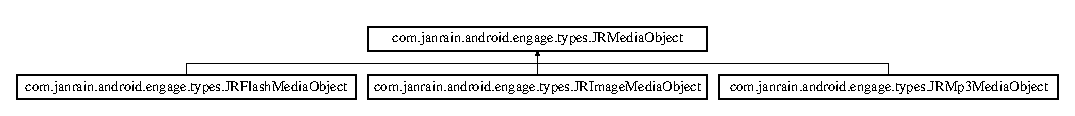
\includegraphics[height=1.107814cm]{classcom_1_1janrain_1_1android_1_1engage_1_1types_1_1_j_r_media_object}
\end{center}
\end{figure}


\subsection{Detailed Description}
Base class for \hyperlink{classcom_1_1janrain_1_1android_1_1engage_1_1types_1_1_j_r_image_media_object}{JRImageMediaObject}, \hyperlink{classcom_1_1janrain_1_1android_1_1engage_1_1types_1_1_j_r_flash_media_object}{JRFlashMediaObject}, and \hyperlink{classcom_1_1janrain_1_1android_1_1engage_1_1types_1_1_j_r_mp3_media_object}{JRMp3MediaObject}. 

The documentation for this class was generated from the following file:\begin{DoxyCompactItemize}
\item 
/Users/lillialexis/Android/engage.android/JREngage/src/com/janrain/android/engage/types/JRMediaObject.java\end{DoxyCompactItemize}

\hypertarget{classcom_1_1janrain_1_1android_1_1engage_1_1types_1_1_j_r_mp3_media_object}{
\section{JRMp3MediaObject Class Reference}
\label{classcom_1_1janrain_1_1android_1_1engage_1_1types_1_1_j_r_mp3_media_object}\index{com::janrain::android::engage::types::JRMp3MediaObject@{com::janrain::android::engage::types::JRMp3MediaObject}}
}


Mp3 object to be included in a post to a user's stream.  




Inherits com::janrain::android::engage::types::JRMediaObject.

\subsection*{Public Member Functions}
\begin{Indent}{\bf Constructors}\par
{\em \label{_amgrp559a25fdb98a7d1fd1c3771ac568d5e9}
 }\begin{DoxyCompactItemize}
\item 
\hyperlink{classcom_1_1janrain_1_1android_1_1engage_1_1types_1_1_j_r_mp3_media_object_af0943c007a4be987b3441b4317061306}{JRMp3MediaObject} (String src)
\item 
\hypertarget{classcom_1_1janrain_1_1android_1_1engage_1_1types_1_1_j_r_mp3_media_object_a942f1490911b90f61fcc82f4f0674838}{
String {\bfseries getSrc} ()}
\label{classcom_1_1janrain_1_1android_1_1engage_1_1types_1_1_j_r_mp3_media_object_a942f1490911b90f61fcc82f4f0674838}

\item 
\hypertarget{classcom_1_1janrain_1_1android_1_1engage_1_1types_1_1_j_r_mp3_media_object_a888f94790c968e3f0b5de17e509098aa}{
String {\bfseries getTitle} ()}
\label{classcom_1_1janrain_1_1android_1_1engage_1_1types_1_1_j_r_mp3_media_object_a888f94790c968e3f0b5de17e509098aa}

\item 
\hypertarget{classcom_1_1janrain_1_1android_1_1engage_1_1types_1_1_j_r_mp3_media_object_a7d4a73d6a1db487dd96f658bdbc98ae9}{
void {\bfseries setTitle} (String title)}
\label{classcom_1_1janrain_1_1android_1_1engage_1_1types_1_1_j_r_mp3_media_object_a7d4a73d6a1db487dd96f658bdbc98ae9}

\item 
\hypertarget{classcom_1_1janrain_1_1android_1_1engage_1_1types_1_1_j_r_mp3_media_object_a1b9f565753d008491c59887680bd570e}{
String {\bfseries getArtist} ()}
\label{classcom_1_1janrain_1_1android_1_1engage_1_1types_1_1_j_r_mp3_media_object_a1b9f565753d008491c59887680bd570e}

\item 
\hypertarget{classcom_1_1janrain_1_1android_1_1engage_1_1types_1_1_j_r_mp3_media_object_ad3502580239a5b59adb83dbbd4651fe4}{
void {\bfseries setArtist} (String artist)}
\label{classcom_1_1janrain_1_1android_1_1engage_1_1types_1_1_j_r_mp3_media_object_ad3502580239a5b59adb83dbbd4651fe4}

\item 
\hypertarget{classcom_1_1janrain_1_1android_1_1engage_1_1types_1_1_j_r_mp3_media_object_a11ac7b770ff2135e877c241ddb5db662}{
String {\bfseries getAlbum} ()}
\label{classcom_1_1janrain_1_1android_1_1engage_1_1types_1_1_j_r_mp3_media_object_a11ac7b770ff2135e877c241ddb5db662}

\item 
\hypertarget{classcom_1_1janrain_1_1android_1_1engage_1_1types_1_1_j_r_mp3_media_object_a90033ebe6c28a946a4c88965365961fb}{
void {\bfseries setAlbum} (String album)}
\label{classcom_1_1janrain_1_1android_1_1engage_1_1types_1_1_j_r_mp3_media_object_a90033ebe6c28a946a4c88965365961fb}

\item 
\hypertarget{classcom_1_1janrain_1_1android_1_1engage_1_1types_1_1_j_r_mp3_media_object_a68adac94351807681f1b2828b9c68734}{
String {\bfseries getType} ()}
\label{classcom_1_1janrain_1_1android_1_1engage_1_1types_1_1_j_r_mp3_media_object_a68adac94351807681f1b2828b9c68734}

\end{DoxyCompactItemize}
\end{Indent}
\subsection*{Private Attributes}
\begin{DoxyCompactItemize}
\item 
String \hyperlink{classcom_1_1janrain_1_1android_1_1engage_1_1types_1_1_j_r_mp3_media_object_a55bae62e4521511e834270cbb7910aa6}{mSrc}
\item 
String \hyperlink{classcom_1_1janrain_1_1android_1_1engage_1_1types_1_1_j_r_mp3_media_object_a6a07e9575c466f0cfeb02907ae8d0973}{mTitle}
\item 
String \hyperlink{classcom_1_1janrain_1_1android_1_1engage_1_1types_1_1_j_r_mp3_media_object_a447e5238acd3b656ad1658af4d1d585b}{mArtist}
\item 
String \hyperlink{classcom_1_1janrain_1_1android_1_1engage_1_1types_1_1_j_r_mp3_media_object_a0beebc1720c6f4bcf3190b3a112658b4}{mAlbum}
\end{DoxyCompactItemize}


\subsection{Detailed Description}
Mp3 object to be included in a post to a user's stream. Create an mp3 media object, fill in the object's fields, and add the object to the JRActivityObject.media array in your \hyperlink{classcom_1_1janrain_1_1android_1_1engage_1_1types_1_1_j_r_activity_object}{JRActivityObject}. How the mp3s get presented and whether or not they are used, depend on the provider.

Each mp3 must contain a {\itshape src\/} url, which is the URL of the MP3 file to be rendered. The mp3 can also include a {\itshape title\/}, {\itshape artist\/}, and {\itshape album\/}.

\begin{DoxyNote}{Note}
You can only include one \hyperlink{classcom_1_1janrain_1_1android_1_1engage_1_1types_1_1_j_r_mp3_media_object}{JRMp3MediaObject} in the media array. Any others will be ignored.
\end{DoxyNote}
$\ast$ @ Format and rules are identical to those described on the \href{http://developers.facebook.com/docs/guides/attachments}{\tt Facebook Developer page on Attachments}. 

\subsection{Constructor}
\hypertarget{classcom_1_1janrain_1_1android_1_1engage_1_1types_1_1_j_r_mp3_media_object_af0943c007a4be987b3441b4317061306}{
\index{com::janrain::android::engage::types::JRMp3MediaObject@{com::janrain::android::engage::types::JRMp3MediaObject}!JRMp3MediaObject@{JRMp3MediaObject}}
\index{JRMp3MediaObject@{JRMp3MediaObject}!com::janrain::android::engage::types::JRMp3MediaObject@{com::janrain::android::engage::types::JRMp3MediaObject}}
\subsubsection[{JRMp3MediaObject}]{\setlength{\rightskip}{0pt plus 5cm}{\bf JRMp3MediaObject} (
\begin{DoxyParamCaption}
\item[{String}]{ src}
\end{DoxyParamCaption}
)}}
\label{classcom_1_1janrain_1_1android_1_1engage_1_1types_1_1_j_r_mp3_media_object_af0943c007a4be987b3441b4317061306}
Returns a {\ttfamily \hyperlink{classcom_1_1janrain_1_1android_1_1engage_1_1types_1_1_j_r_mp3_media_object}{JRMp3MediaObject}} initialized with the given src.


\begin{DoxyParams}{Parameters}
\item[{\em src}]The URL of the MP3 file to be rendered. This value cannot be {\ttfamily nil}.\end{DoxyParams}
\begin{DoxyReturn}{Returns}
A \hyperlink{classcom_1_1janrain_1_1android_1_1engage_1_1types_1_1_j_r_mp3_media_object}{JRMp3MediaObject} initialized with the given src. If {\ttfamily src} is {\itshape nil\/}, returns {\ttfamily nil}.
\end{DoxyReturn}

\begin{DoxyExceptions}{Exceptions}
\item[{\em IllegalArgumentException}]if src is null \end{DoxyExceptions}


\subsection{Variables}
\hypertarget{classcom_1_1janrain_1_1android_1_1engage_1_1types_1_1_j_r_mp3_media_object_a55bae62e4521511e834270cbb7910aa6}{
\index{com::janrain::android::engage::types::JRMp3MediaObject@{com::janrain::android::engage::types::JRMp3MediaObject}!mSrc@{mSrc}}
\index{mSrc@{mSrc}!com::janrain::android::engage::types::JRMp3MediaObject@{com::janrain::android::engage::types::JRMp3MediaObject}}
\subsubsection[{mSrc}]{\setlength{\rightskip}{0pt plus 5cm}String {\bf mSrc}\hspace{0.3cm}{\ttfamily  \mbox{[}private\mbox{]}}}}
\label{classcom_1_1janrain_1_1android_1_1engage_1_1types_1_1_j_r_mp3_media_object_a55bae62e4521511e834270cbb7910aa6}
The URL of the MP3 file to be rendered \hypertarget{classcom_1_1janrain_1_1android_1_1engage_1_1types_1_1_j_r_mp3_media_object_a6a07e9575c466f0cfeb02907ae8d0973}{
\index{com::janrain::android::engage::types::JRMp3MediaObject@{com::janrain::android::engage::types::JRMp3MediaObject}!mTitle@{mTitle}}
\index{mTitle@{mTitle}!com::janrain::android::engage::types::JRMp3MediaObject@{com::janrain::android::engage::types::JRMp3MediaObject}}
\subsubsection[{mTitle}]{\setlength{\rightskip}{0pt plus 5cm}String {\bf mTitle}\hspace{0.3cm}{\ttfamily  \mbox{[}private\mbox{]}}}}
\label{classcom_1_1janrain_1_1android_1_1engage_1_1types_1_1_j_r_mp3_media_object_a6a07e9575c466f0cfeb02907ae8d0973}
The title of the song \hypertarget{classcom_1_1janrain_1_1android_1_1engage_1_1types_1_1_j_r_mp3_media_object_a447e5238acd3b656ad1658af4d1d585b}{
\index{com::janrain::android::engage::types::JRMp3MediaObject@{com::janrain::android::engage::types::JRMp3MediaObject}!mArtist@{mArtist}}
\index{mArtist@{mArtist}!com::janrain::android::engage::types::JRMp3MediaObject@{com::janrain::android::engage::types::JRMp3MediaObject}}
\subsubsection[{mArtist}]{\setlength{\rightskip}{0pt plus 5cm}String {\bf mArtist}\hspace{0.3cm}{\ttfamily  \mbox{[}private\mbox{]}}}}
\label{classcom_1_1janrain_1_1android_1_1engage_1_1types_1_1_j_r_mp3_media_object_a447e5238acd3b656ad1658af4d1d585b}
The artist \hypertarget{classcom_1_1janrain_1_1android_1_1engage_1_1types_1_1_j_r_mp3_media_object_a0beebc1720c6f4bcf3190b3a112658b4}{
\index{com::janrain::android::engage::types::JRMp3MediaObject@{com::janrain::android::engage::types::JRMp3MediaObject}!mAlbum@{mAlbum}}
\index{mAlbum@{mAlbum}!com::janrain::android::engage::types::JRMp3MediaObject@{com::janrain::android::engage::types::JRMp3MediaObject}}
\subsubsection[{mAlbum}]{\setlength{\rightskip}{0pt plus 5cm}String {\bf mAlbum}\hspace{0.3cm}{\ttfamily  \mbox{[}private\mbox{]}}}}
\label{classcom_1_1janrain_1_1android_1_1engage_1_1types_1_1_j_r_mp3_media_object_a0beebc1720c6f4bcf3190b3a112658b4}
The album 

The documentation for this class was generated from the following file:\begin{DoxyCompactItemize}
\item 
/Users/lillialexis/Android/engage.android/JREngage/src/com/janrain/android/engage/types/JRMp3MediaObject.java\end{DoxyCompactItemize}

\printindex
\end{document}
